\chapter{Estudio espectral}
\label{chap: estudio espectral}


\section{Motivación para realizar un estudio espectral de los PDL}
No es difícil convencerse de que las condiciones de ortogonalidad
impuestas en la definición de la base discreta de Legendre
\marginnote{En esta motivación informal, por oscilación
de una señal $x = (x_{m})_{m=0}^{n-1}$
entendemos
tres cambios consecutivos de signo en sus entradas.}
$\cali{L}^{n}$
forzan a las entradas de los polinomios discretos $\cali{L}^{n,k}$
a cambiar más frecuentemente de signo conforme aumenta
el grado $k$, luego, conforme $k$ tiende a $n-1$,
la cantidad de oscilaciones aumenta; revisemos, 
por ejemplo, el caso $n=4$.



\begin{minipage}{0.5\textwidth}
\begin{figure}[H]
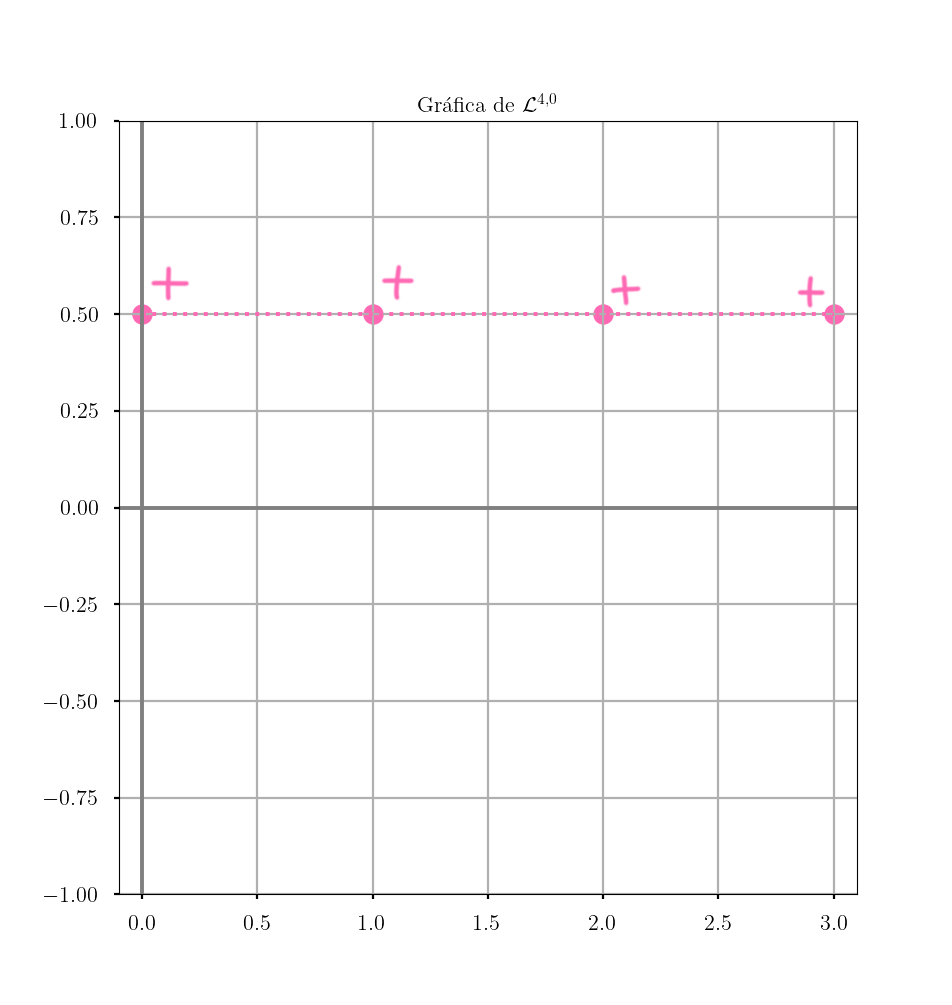
\includegraphics[scale=0.25]{oscil1}
\end{figure}
\end{minipage} \hfill
\begin{minipage}{0.45\textwidth}
1.- Por definición,
$\mathcal{L}^{4,0}$ se obtiene al normalizar 
al vector constante uno de $\IR^{4}$, o sea, 

\[
\cali{L}^{4,0} = \left(
\frac{1}{2}, \frac{1}{2}, \frac{1}{2}, \frac{1}{2}
\right).
\]
\end{minipage} 


\begin{minipage}{0.5\textwidth}
2.- La señal $\cali{L}^{4,1} \in \IR^{4}$ es un polinomio discreto de
dimensión 4 y grado 1 que se obtiene exigiendo las
siguientes condiciones

\[
\langle \cali{L}^{4,1} , \cali{L}^{4,0} \rangle=0
\hspace{0.2cm} \text{y} \hspace{0.2cm}
\langle \cali{L}^{4,1} , \cali{L}^{4,1} \rangle=1;
\]
esta primera condición se refleja en que 
las alturas de los puntos de la gráfica de 
$\cali{L}^{4,1}$ deben sumar cero;
esto implica un cambio de signo (y sólo uno,
pues el polinomio es lineal).

\end{minipage} \hfill
\begin{minipage}{0.45\textwidth}
\begin{figure}[H]
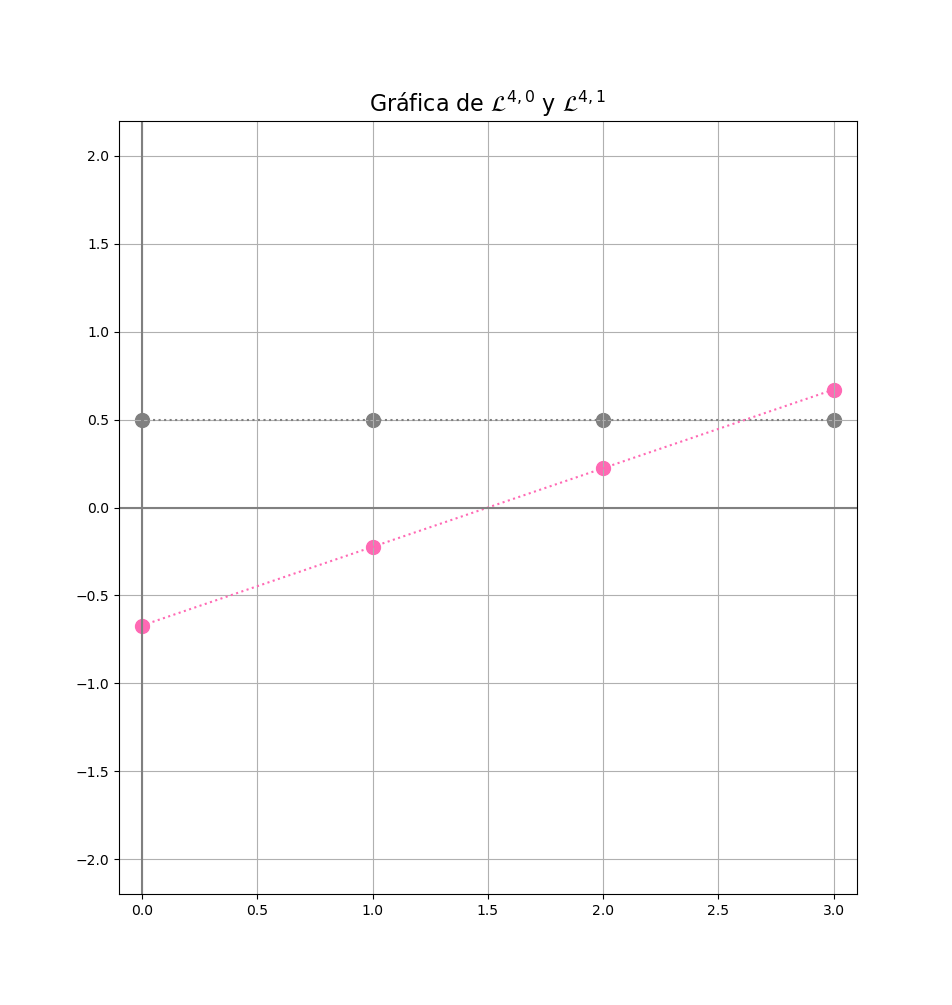
\includegraphics[scale=0.3]{oscil2}
\end{figure}
\end{minipage}

\noindent
3.- El vector
$\cali{L}^{4,2} \in \IR^{4}$,
que es un polinomio discreto
de grado $2$, satisface las siguientes
tres condiciones:

\[
\langle \cali{L}^{4,2} , \cali{L}^{4,0} \rangle=0,
\hspace{0.2cm}
\langle \cali{L}^{4,2} , \cali{L}^{4,1} \rangle=0,
\hspace{0.2cm} \text{y} \hspace{0.2cm}
\langle \cali{L}^{4,2} , \cali{L}^{4,2} \rangle=1.
\]
La segunda condición no da información sobre más
requerimientos que deba cumplir
$\cali{L}^{4,2}$, pues,
como $\cali{L}^{4,1} \in S_{n,-}$
y $\cali{L}^{4,2} \in S_{n,+}$
(c.f. teorema 
\ref{prop: simetrias en dimensiones pares}),
ya del lema
\ref{lema: ortogonalidad entre sim y antisim}
se deducía la ortogonalidad de estas señales; 
observe sin embargo que, si las entradas de 
$\cali{L}^{4,2}$ fuesen todas positivas o todas negativas,
entonces no se tendría la ortogonalidad
con la señal constante $\cali{L}^{4,0}$.


\begin{figure}[H]
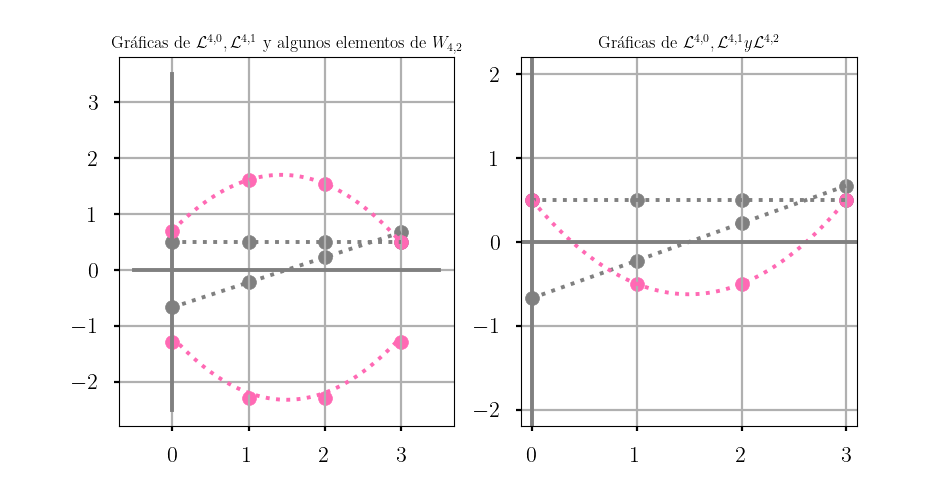
\includegraphics[scale=0.6]{oscil3}
\end{figure}

4.- Por último, $\cali{L}^{4,3} \in \IR^{4}$ satisface
las siguientes cuatro condiciones: 

\[
\langle \cali{L}^{4,3} , \cali{L}^{4,0} \rangle=0,
\hspace{0.2cm}
\langle \cali{L}^{4,3} , \cali{L}^{4,1} \rangle=0,
\langle \cali{L}^{4,3} , \cali{L}^{4,2} \rangle=0,
\hspace{0.2cm} \text{y} \hspace{0.2cm}
\langle \cali{L}^{4,3} , \cali{L}^{4,3} \rangle=1.
\]

Según los teoremas 
\ref{cor: propiedades importantes de espacios Wi}
y \ref{prop: simetrias en dimensiones pares},
$\cali{L}^{4,3}$ es la discretización de un polinomio
cúbico y además es una señal antisimétrica (en el sentido de la definición
\ref{def: espacios de seniales simetricas y antisimetricas}); dos gráficas de señales que cumplen esto se ilustran abajo:

\begin{figure}[H]
	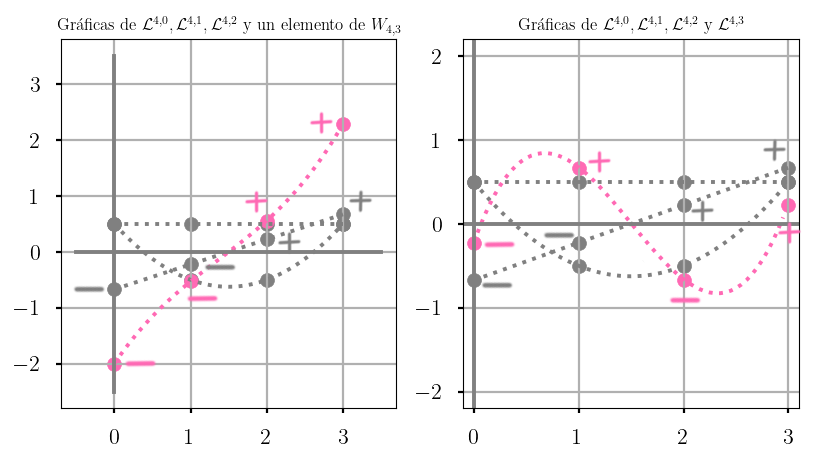
\includegraphics[scale=0.6]{oscil4}
	\sidecaption{Observe que la señal cúbica de la izquierda tiene
	un sólo cambio de signo, mientras que la de la derecha (que es 
	$\cali{L}^{4,3}$) tiene tres.}
\end{figure}

La señal cúbica de la izquierda, a pesar de 
ser ortogonal a $\mathcal{L}^{4,0}$ y a $\cali{L}^{4,2}$ por 
simetría (c.f. lema
\ref{lema: ortogonalidad entre sim y antisim}), 
definitivamente no puede ser ortogonal
a $\cali{L}^{4,1}$, pues las entradas de estos dos vectores de 
$\IR^{4}$ tienen el mismo signo. Sin embargo, la señal cúbica 
de la derecha (que de hecho es $\cali{L}^{4,3}$) sí cumple el ser
ortogonal a $\cali{L}^{4,1}$ pero, para lograr esto, sus
entradas deben cambiar de signo tres veces. \\

\section{Hipótesis sobre las oscilaciones de los PDL}

Estando de acuerdo en que es pertinente realizar un análisis
espectral de los PDL, después de dibujar las gráficas de algunos
de estos para varias dimensiones $n$, proponemos una hipótesis
que relaciona una presencia importante de cierta frecuencia
de oscilación asociada a un PDL.


\begin{figure}[H]
	\sidecaption{
	Aproximando las gráficas
	de $\cali{L}^{60,0}$ y $\cali{L}^{60,1}$
	con sinusoides. 
	\label{fig: hip_0,1}
	}
	\centering
	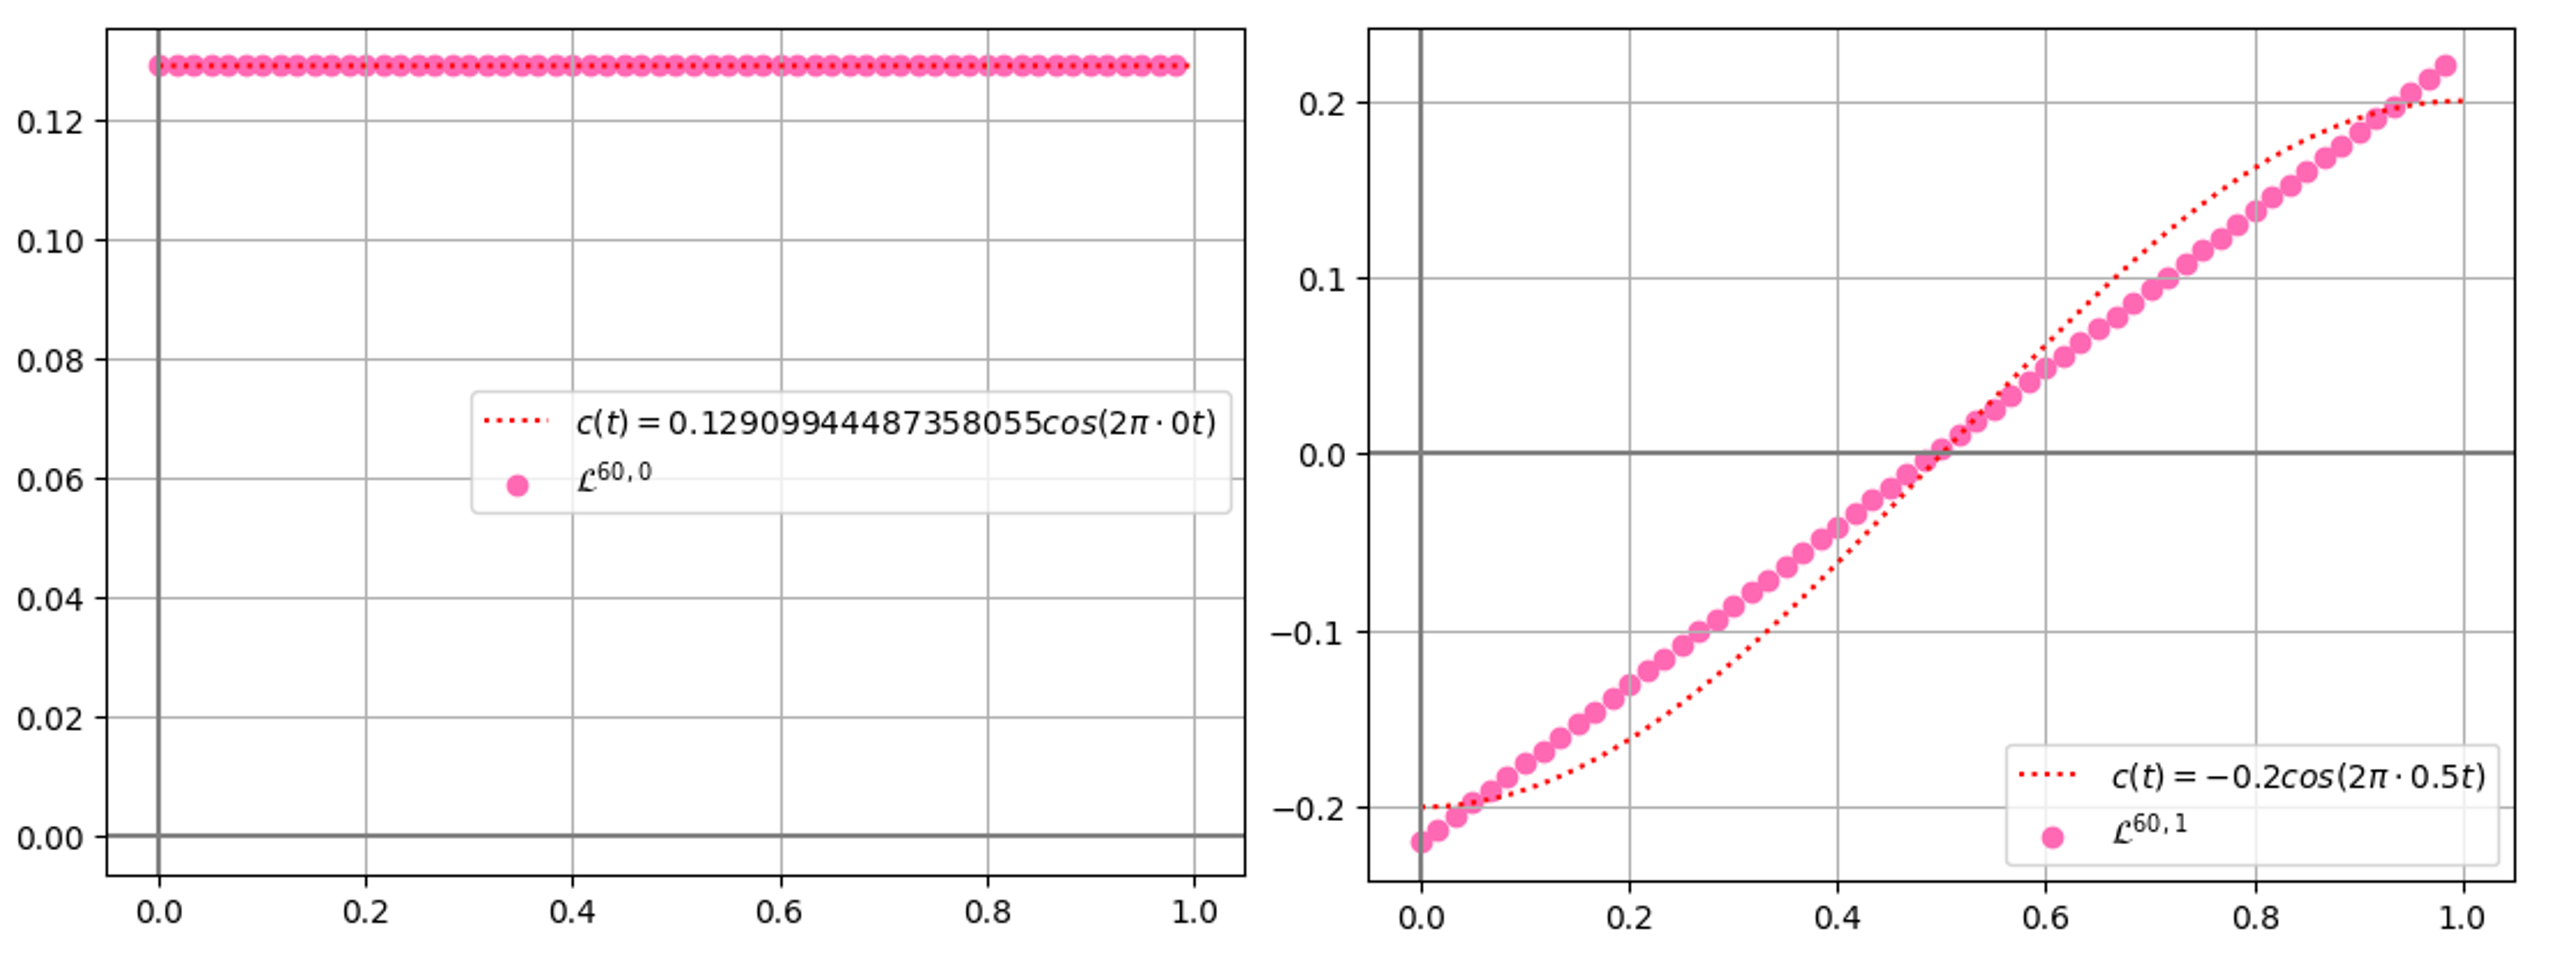
\includegraphics[scale = 0.6]{hip_0,1} 
\end{figure}	

\begin{figure}[H]
	\sidecaption{
	Aproximando las gráficas
	de $\cali{L}^{60,2}$ y $\cali{L}^{60,3}$
	con sinusoides. 
	\label{fig: hip_2,3}
	}
	\centering
	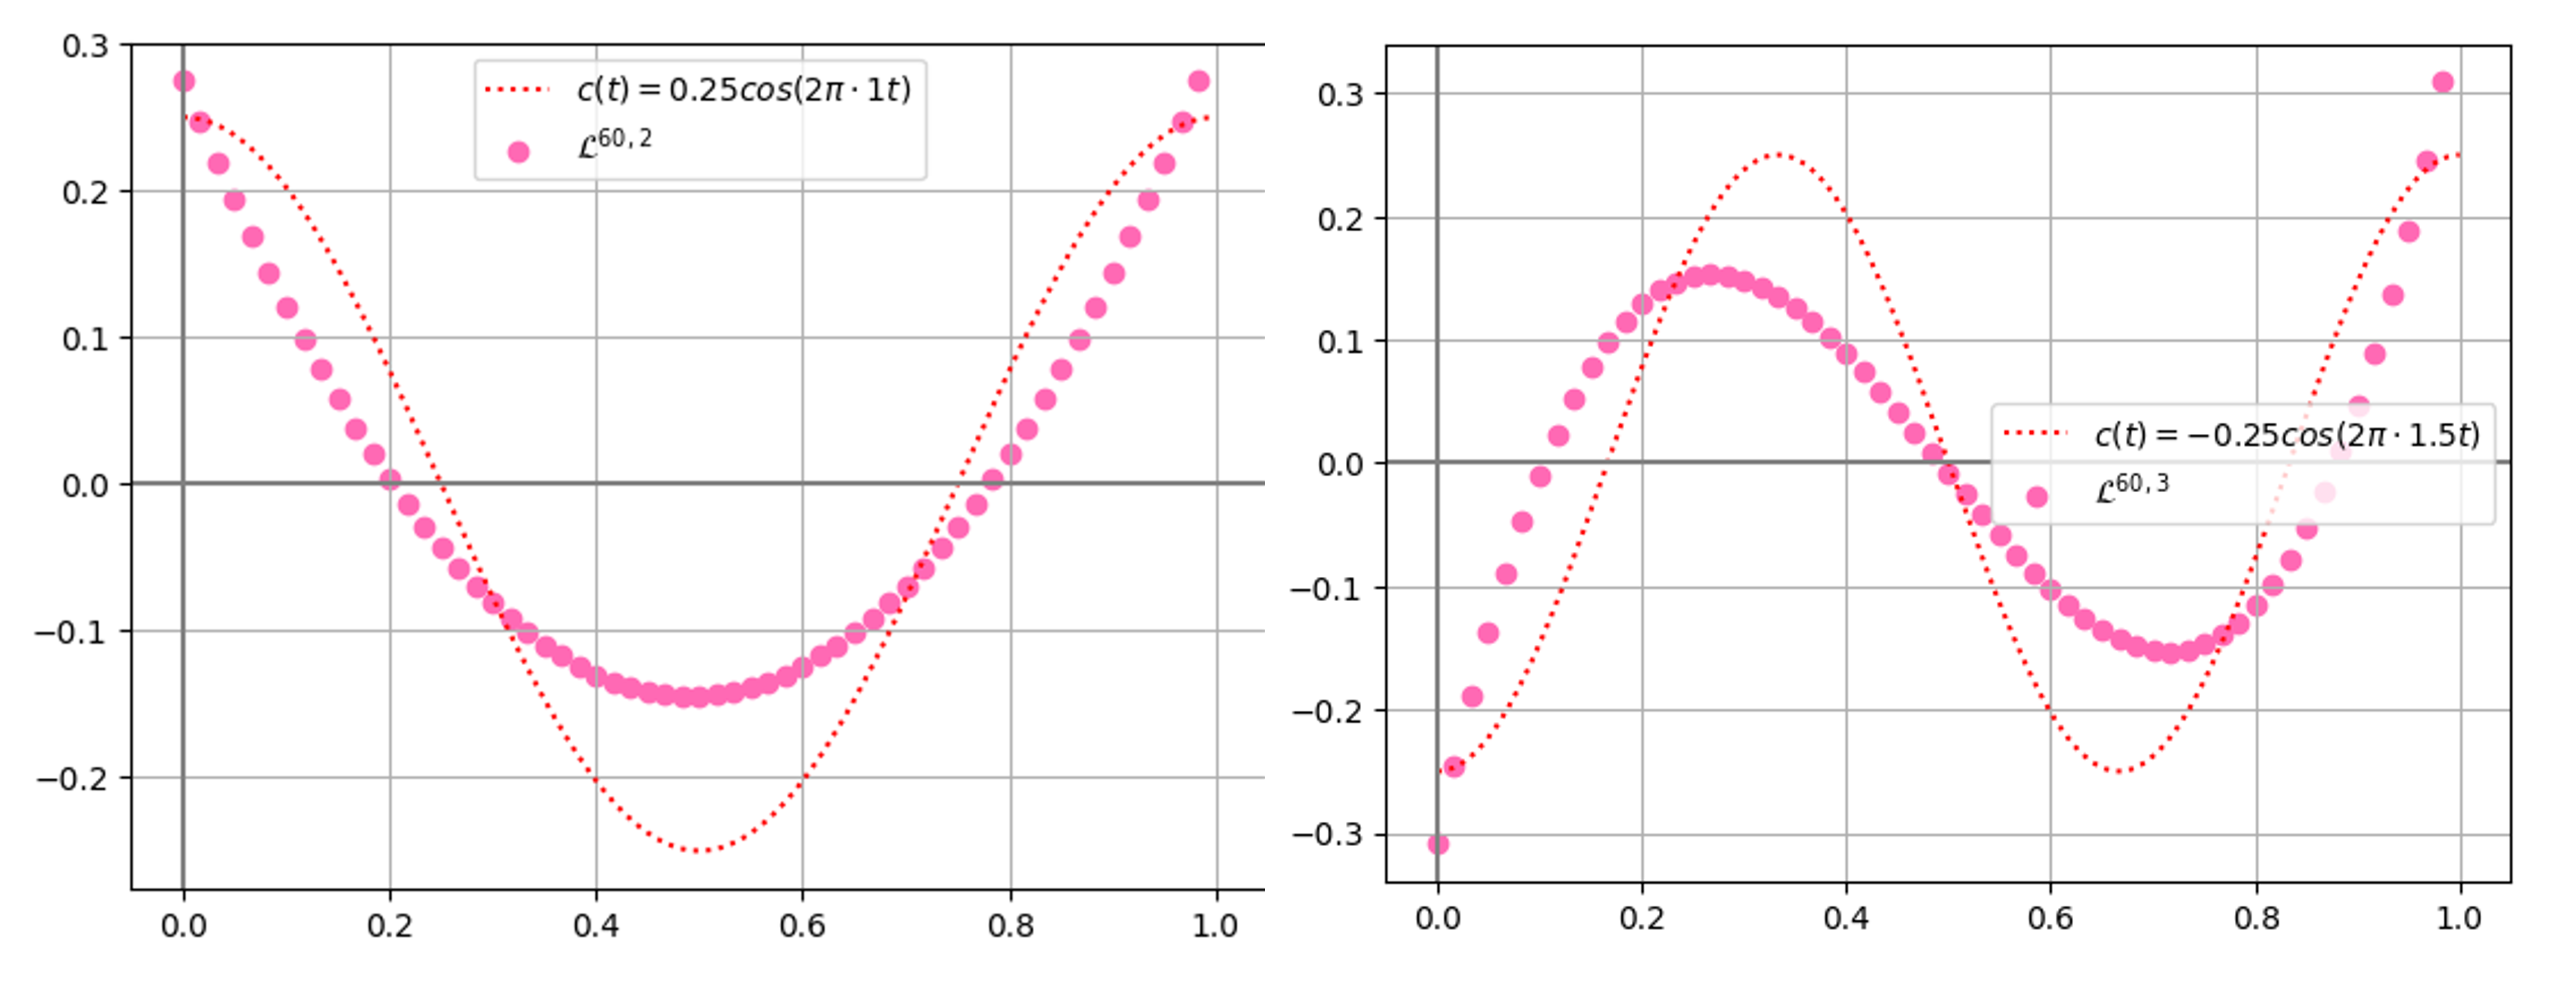
\includegraphics[scale = 0.6]{hip_2,3} 
\end{figure}	

\begin{figure}[H]
	\sidecaption{
	Aproximando las gráficas
	de $\cali{L}^{60,4}$ y $\cali{L}^{60,5}$
	con sinusoides. 
	\label{fig: hip_4,5}
	}
	\centering
	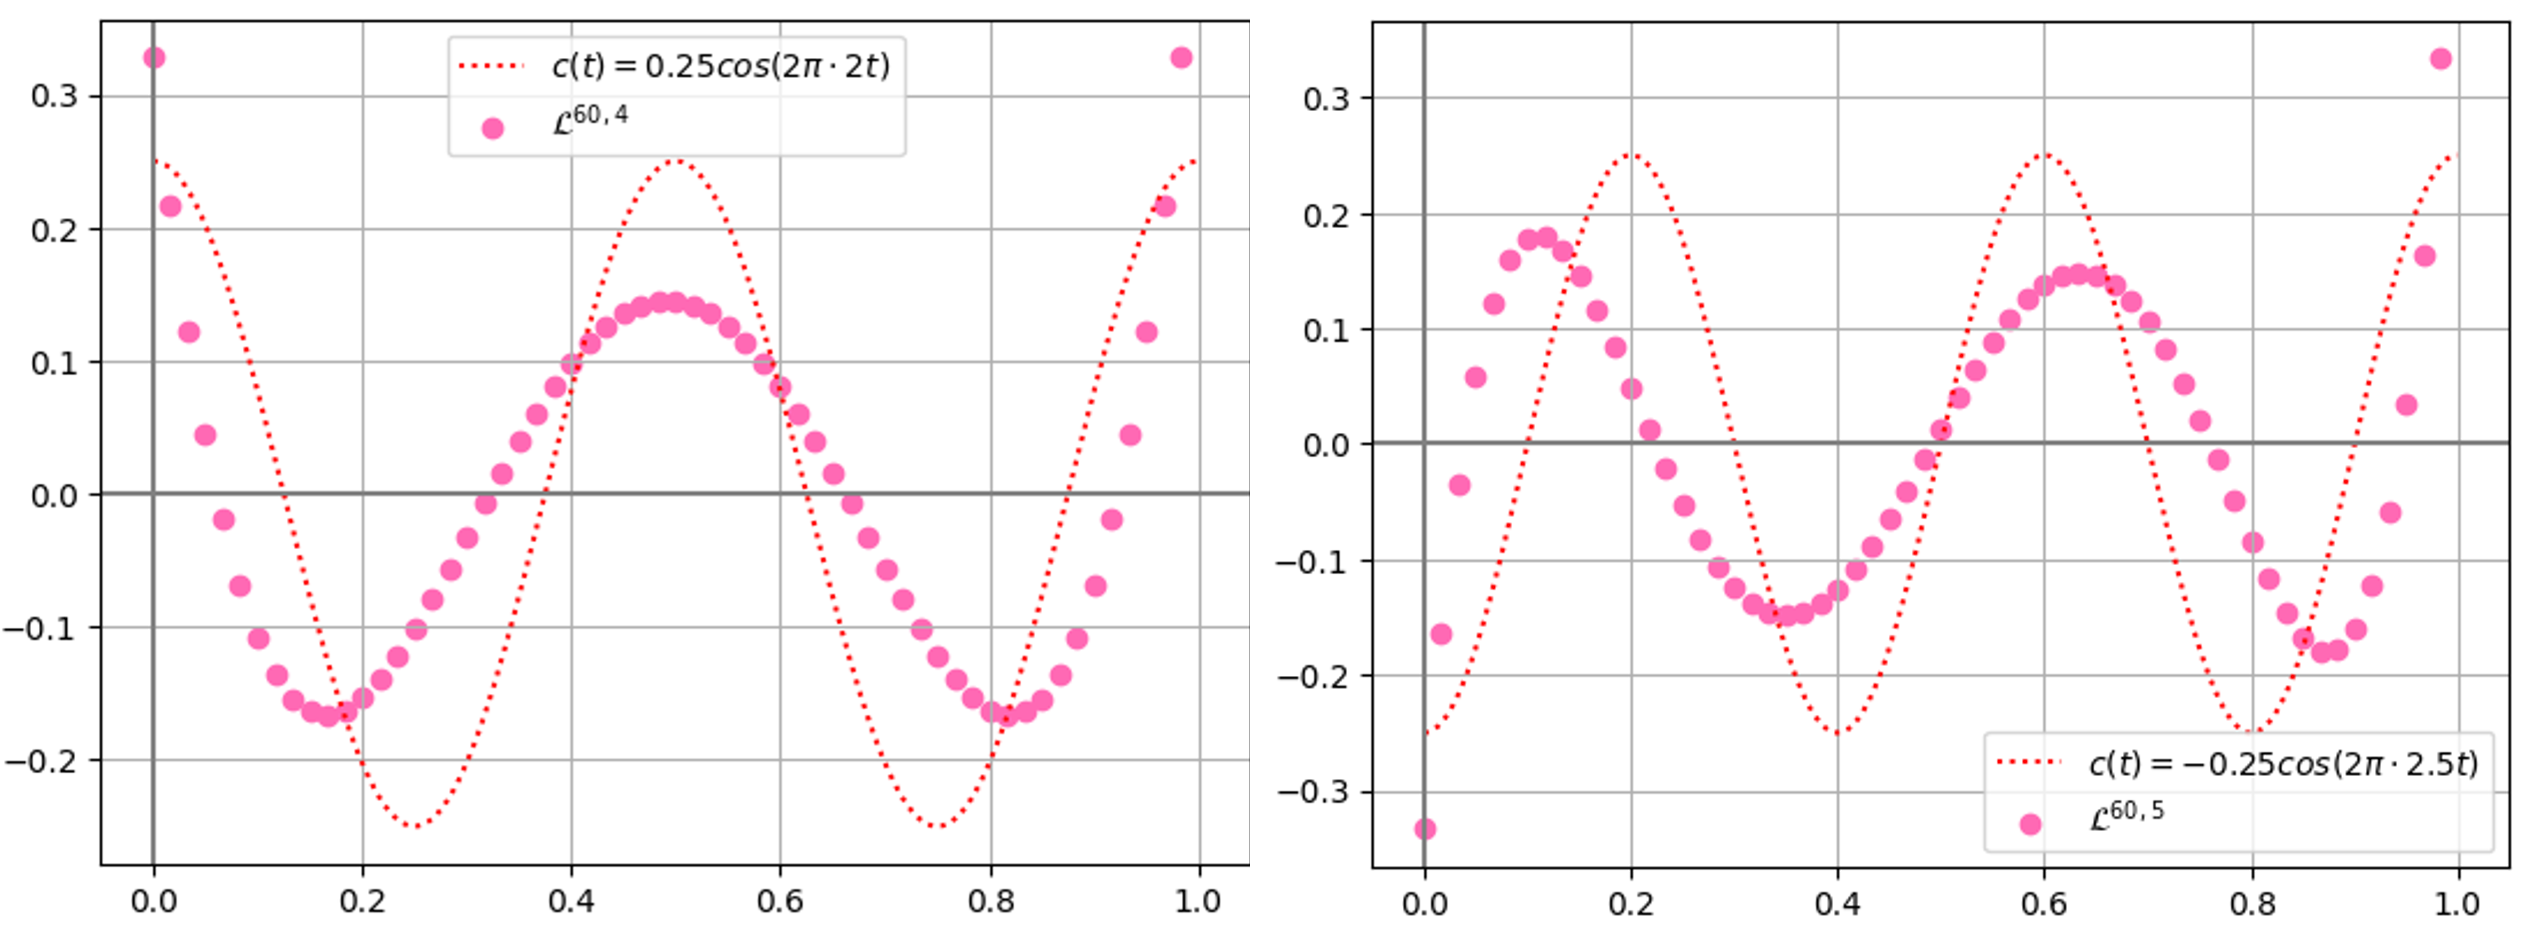
\includegraphics[scale = 0.6]{hip_4,5} 
\end{figure}	

\begin{hip}
\label{ref: hipotesis}
Sean $n \geq 2$, $0 \leq k \leq n-1$ entero. 
Sea $\cali{L}^{n,k}$ el PDL de dimensión $n$ y grado $k$.
La frecuencia que mejor modela la oscilación de la gráfica
de $\cali{L}^{n,k}$ es $\frac{k}{2}$ 
\end{hip}

Se ha formulado de forma intencional la hipótesis 
\ref{ref: hipotesis} en términos vagos, para tener libertad
después de definir las herramientas con las que abordaremos el problema
de dar forma concreta a la hipótesis y mejorarla o refutarla con simulaciones
numéricas.

\section{La transformada discreta de Fourier}
\label{sec: TDF}

En esta sección vamos a dar la definición usual de 
las bases de Fourier complejas y reales, que son
bases ortonormales de $\IC^{n}$ y de $\IR^{n}$ 
\marginnote{Incluimos este capítulo de teoría clásica
por completitud de este trabajo
y para fijar la notación. 
\cite{fourier1} y \cite{fourier2}
son referencias con mucha más información.}
de $\IC^{n}$
y una de $\IR^{n}$ (que llamaremos
``bases de Fourier complejas y reales''),
definidas ambas en términos de discretizaciones de
sinusoides de frecuencias enteras, y que son herramientas
clásicas para hacer lo que comúnmente se denomina
un \textbf{análisis espectral} de señales finitas.


Puesto que la definición de estas herramientas requiere
de algunas nociones del análisis complejo (en particular, de la
definición de la exponencial compleja y de las raíces $n-$ésimas
de la unidad), damos brevemente algunas definiciones y resultados
necesarios para definir las bases de Fourier.


\subsection{La exponencial compleja y raíces $n-$ésimas de la unidad}


La definición de la función exponencial compleja 
tiene diversas motivaciones
(puede consultar algunas de estas en 
\cite{marsden}). Nosotros sólo
damos la definición de esta, así como algunas propiedades
de ella que se usarán en lo que sigue.

\begin{defi}
\label{def: exponencial compleja}
Si $y \in \IR$, entonces por $exp(iy)$ denotamos al número
complejo de módulo uno y argumento $y$, es decir,
\begin{equation}
\label{eq: exponencial 1}
exp(iy) := cos(y) + i sen(y).
\end{equation}
Para todo número complejo $z = a+bi$, definimos 
$exp(z)$ como sigue:
\begin{equation}
\label{eq: exponencial 2}
exp(z) := e^{x}(cos(y) + i sen(y)).
\end{equation}
\end{defi}

\begin{prop}
\label{prop: propiedades exp compleja}
(\textbf{Algunas propiedades de la exponencial compleja}) 
Sean $z_{1}, z_{2} \in \IC$, $\omega \in \IZ$.
	\begin{itemize}
	\item $\frac{exp(z_{1})}{exp(z_{2})} = exp(z_{1} - z_{2})$
	\item $exp(z_{1} + z_{2}) = exp(z_{1}) \cdot exp(z_{2})$
	\item $(exp(z_{1}))^{\omega} = exp(\omega z)$
	\item $exp(z) = 1$ si y sólo si $z= 2K \pi i$ para algún $K \in \IZ$ 
	\item para todo $y \in \IR$, 
	\begin{equation}
	\label{eq: coseno exponenciales}
	cos(y) = \frac{exp(iy)+exp(-iy)}{2}
	\end{equation}
	y
	\begin{equation}
	\label{eq: seno exponenciales}
	sen(y) = \frac{exp(iy)-exp(-iy)}{2i}.
	\end{equation}
	\end{itemize}
\end{prop}

\begin{defi}
\label{defi: raices n esimas de la unidad}
Sea $n \in \IN$. A las $n$ raíces complejas del polinomio
$p_{n}(t)= t^{n}-1 \in \IC[t]$ 
se les denominará las \textbf{raíces $n-$ésimas de la unidad.}
\end{defi}


Las raíces $n-$ésimas de la unidad son pues los números complejos
tales que, elevados a la potencia $n$, son iguales a 1; según el 
teorema fundamental
del álgebra \ref{teo: fundamental del algebra}, sí hay números complejos
que satisfacen la definición \ref{defi: raices n esimas de la unidad}, y además
son a lo más $n$. Es fácil establecer, como hacemos a continuación, 
fórmulas explícitas para estos números, que de hecho son exactamente $n$.

\begin{prop}
Sea $n \in \IN$, $n \geq 2$. Hay exactamente $n$ raíces $n-$ésimas de la
unidad, y estas son los números complejos
 	\begin{equation}
	\label{eq3: 8ab}
	z_{n, \omega} : = exp \left( \frac{2 \pi i }{n} \omega
	\right), \hspace*{0.2cm} \textit{con} 
	\hspace*{0.2cm} \omega \in \{0, 1, \ldots, n-1 \}.
	\end{equation}
	
\end{prop}
\noindent
\textbf{Demostración.}
Por las propiedades expresadas en la proposición
\ref{prop: propiedades exp compleja}, es fácil ver que 
$z_{n,1} :=  exp \left( \frac{2 \pi i }{n} \right)$ es raíz $n-$ésima
de la unidad, pues
\[
(z_{n,1})^{n} = exp(2 \pi i ) = 1.
\]
Además, para todo $\omega \in \{ 0, \cdots , n-1 \}$, el número
\[
z_{n, \omega} : = (z_{n,1})^{\omega} = exp \left( \frac{2 \pi i }{n} \omega \right)
\]
también es es raíz $n-$ésima de la unidad, ya que

\[
(z_{n, \omega})^{n} = ((z_{n,1})^{\omega} )^{n} = 
((z_{n,1})^{n} )^{\omega} = 1^{\omega}=1. 
\]
Note ahora que los $n$ números complejos $z_{n, \omega}$ son todos 
distintos entre sí, pues si $\omega_{1}$ y $\omega_{2}$ son enteros
entre $0$ y $n-1$ tales que $z_{n, \omega_{1}} = z_{n, \omega_{2}}$,
o sea, tales que 
$exp \left( \frac{2 \pi i }{n} \omega_{1} \right) = 
exp \left( \frac{2 \pi i }{n} \omega_{1} \right)$, entonces, según el primer
punto de la proposición \ref{prop: propiedades exp compleja},
$1 = exp \left( \frac{2 \pi i }{n} (\omega_{1}-\omega_{2}) \right)$, luego, 
según el cuarto punto de esta misma proposición, $\frac{\omega_{1}-\omega_{2}}{n}$
es entero, o sea, $n$ divide a $\omega_{1}-\omega_{2}$; por el rango de 
$\omega_{1}$ y $\omega_{2}$, esto sólo ocurre si $\omega_{1}-\omega_{2}$ es
cero, o sea, si $\omega_{1}$ y $\omega_{2}$
son iguales.
\QEDB
\vspace{0.2cm}

\begin{figure}[H]
	\sidecaption{
	Para construir gráficamente a las raíces $n-$ésimas de la
	unidad, se debe dividir, a partir del punto $(0,1)$, a la
	circunferencia unitaria en $n$ partes iguales. Según esta construcción
	y la interpretación geométrica de la multiplicación compleja, es claro
	que multiplicando a $z_{n,1}$ consigo mismo se obtienen a
	todas las demás raíces $n-$ésimas.
	\label{fig: raices unidad}
	}
	\centering
	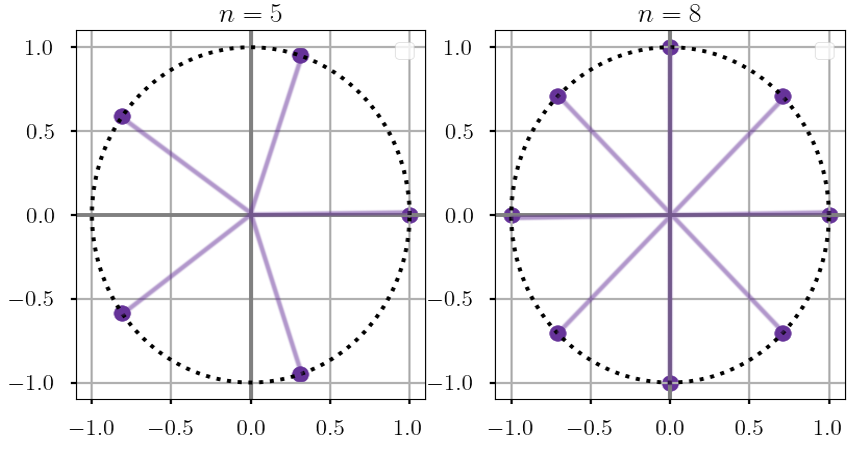
\includegraphics[scale=0.53]{raices_unidad} 
\end{figure}	


\subsection{La transformada discreta de Fourier}

Ya tenemos todo lo necesario para definir a la base
de Fourier compleja de la que hablamos al inicio.
\marginnote{El producto punto que estamos
considerando en el $\IC-$espacio
vectorial $\IC^{n}$ es el que definimos
en \eqref{eq: producto punto Cn}, y el del
$\IR-$espacio vectorial $\IR^{n}$ es el definido en 
\eqref{eq: producto punto Rn}.}

\begin{prop}
\label{prop: construccion Bn}
Sea $n \in \IN$. El conjunto

\begin{equation}
\label{eq2: 8ab}
\cali{B}_{n} : = \left\{
e_{n,\omega} = \left(
\frac{1}{\sqrt{n}} exp \left(
2 \pi i \omega \frac{m}{n}
\right)
\right)_{0 \leq m \leq n-1}
: \hspace{0.2cm} 0 \leq \omega \leq n-1
 \right\}
\end{equation}
es una base ortonormal del $\IC-$espacio
vectorial $\IC^{n}$.
\end{prop}

\noindent
\textbf{Demostración.}
Calculemos el producto punto de dos elementos
$e_{n,\omega_{1}}$ y $e_{n,\omega_{2}}$ del conjunto \eqref{eq2: 8ab};
si $\omega := \omega_{1}-\omega_{2}$,
\begin{align*}
\langle e_{n,w_{1}}, e_{n,w_{2}} \rangle = &
\frac{1}{n}
\suma{m=0}{n-1}{exp \left( 2 \pi i \frac{m}{n} \omega_{1} \right)
\cdot \overline{ exp \left( 2 \pi i \frac{m}{n} \omega_{2} \right) }} \\
= & \frac{1}{n}
\suma{m=0}{n-1}{\left( 2 \pi i \frac{m}{n} (\omega_{1}-\omega_{2}) \right)} \\
= & \frac{1}{n}\suma{m=0}{n-1}{exp\left( 2 \pi i \frac{\omega}{n} m \right)} \\
= & \frac{1}{n}\suma{m=0}{n-1}{exp\left( 2 \pi i \frac{\omega}{n}  \right)^{m}} \\
= & \frac{1}{n}\suma{m=0}{n-1}{(z_{n, \omega})^{m}};
\end{align*}

\noindent
esta última es una suma geométrica. 
\begin{itemize}
	\item Si $\omega_{1} \neq \omega_{2}$, entonces $n$ no puede dividir 
	a $\omega = \omega_{1}-\omega_{2}$ (pues, por el rango en el que se encuentran
	$\omega_{1}$ y $\omega_{2}$, $w \in [-(n-1), n-1]$, y el único múltiplo
	de $n$ en este intervalo es cero), luego, $z_{n, \omega} \neq 1$.
	En este caso se tiene entonces que 
	\[
	\langle e_{n,w_{1}}, e_{n,w_{2}} \rangle = 
	\frac{1}{n}\suma{m=0}{n-1}{(z_{n, \omega})^{m}}
	= \frac{1}{n} \cdot \frac{(z_{n, \omega})^{n}-1}{z_{n, \omega}-1}=
	\frac{1}{n} \cdot \frac{1-1}{z_{n, \omega}-1}=0.
	\]
	
	\item Si $\omega_{1} = \omega_{2}$, entonces $\omega = 0$, y
	\[
	\langle e_{n,w_{1}}, e_{n,w_{2}} \rangle = 
	\frac{1}{n}\suma{m=0}{n-1}{(z_{n, 0})^{m}}
	= \frac{1}{n}\suma{m=0}{n-1}{1} = \frac{1}{n} \cdot n = 1.
	\]
\end{itemize}

Demostramos así que los elementos de $\cali{B}_{n}$
tienen norma uno y que además
son ortogonales
dos a dos, luego, $\cali{B}_{n}$ es un subconjunto l.i. 
de $\IC^{n}$; como $\IC^{n}$ es un $\IC-$espacio vectorial de 
dimensión $n$, concluimos lo deseado.
\QEDB
\vspace{0.2cm}

Por ser \eqref{eq2: 8ab} una BON de $\IC^{n}$, siempre es
posible expresar a un vector $x = (x_{m})_{0 \leq m \leq n-1} \in \IC^{n}$
como combinación lineal de los elementos de \eqref{eq2: 8ab}
y además los coeficientes están dados por los productos punto
de $x$ y los elementos de \eqref{eq2: 8ab}
(c.f. nota \ref{nota: sobre la identidad de parseval}).

\begin{defi}
Sean $n \in \IN$, $x = (x_{m})_{m=0}^{n-1} \in \IC^{n}$
una señal compleja de longitud $n$.
Sea $\cali{B}_{n}$ la base de $\IC^{n}$ definida en 
la proposición \ref{prop: construccion Bn}. \\

A la función $f_{x}: \{ 0, 1, \ldots, n-1 \} 
\rightarrow \IC^{n}$ que a cada
frecuencia $\omega \in \{ 0, 1, \ldots, n-1 \} $
le asocia el coeficiente de $x$ respecto 
al elemento $e_{n, \omega}$ de la base
$\cali{B}_{n}$, o sea, la función definida como
\begin{equation}
\label{eq: TDF}
f_{x}(\omega) = X_{\omega} := 
\frac{1}{\sqrt{n}} \suma{m=0}{n-1}{x_{m} exp \left(
2 \pi i \omega \frac{m}{n}
\right)}
\end{equation}
le llamaremos la 
\textbf{transformada discreta de Fourier de $x$}.
Muchas veces identificamos a tal transformada
con el vector
$X := (X_{\omega})_{\omega = 0}^{n-1}$, que 
no es más que la representación 
de $x = (x_{m})_{m=0}^{n-1}$ respecto a la 
base de frecuencias $\cali{B}_{n}$.
\end{defi}

\marginnote{Por sus siglas en inglés, a la transformada discreta
de Fourier también se le denomina ``TDF''.}


\begin{comment}
{\Huge{\textcolor{red}{TDF}}} 

{\Huge{\textcolor{red}{Dominio: tiempo}}} 


{\Huge{\textcolor{red}{Dominio: frecuencia}}}

{\Huge{ $x = (x_{m})_{0 \leq m \leq n-1}$ }}

{\Huge{ $\langle x, e_{\omega} \rangle$, $0 \leq \omega \leq n-1 $ }}

\end{comment}

Calcular entonces la transformada discreta de Fourier
de $x$ consiste en calcular a los productos
punto $\langle x, e_{n,\omega} \rangle $, que son

\begin{align*}
X_{\omega} := \langle x, e_{n,\omega} \rangle = & 
\frac{1}{\sqrt{n}} \suma{m=0}{n-1}{x_{m} exp \left(
2 \pi i \omega \frac{m}{n}
\right)} \\
= & 
\frac{1}{\sqrt{n}} \suma{m=0}{n-1}{x_{m} 
\left(
exp \left( \frac{2 \pi i }{n} \omega
\right) \right)^{m}} \\
= & A_{x}(z_{n, \omega}),
\end{align*}


\noindent
donde $z_{n, \omega}$ es como en \eqref{eq3: 8ab} y 
$A_{x} = A_{x}(t) \in \IC[t]$ es el polinomio de 
coeficientes complejos definido 
a partir de $x$ como sigue:

	\begin{equation}
		\label{eq4: 8ab}
		A_{x}(t) := \suma{m=0}{n-1}{\frac{x_{m}}{\sqrt{n}} t }\in \IC[t];
	\end{equation}

\noindent
así, \textbf{calcular la transformada
discreta de Fourier de $x$ es lo mismo que evaluar al polinomio 
$A_{x}$ de grado a lo más $n-1$ definido en \eqref{eq4: 8ab} en todas las raíces
$n-$ésimas de la unidad.} 


\begin{nota}
Según este último párrafo, calcular transformadas discretas
de Fourier requiere de algoritmos eficientes para evaluar
polinomios en raíces $n-$ésimas de la unidad. Usando propiedades
de las raíces $n-$ésimas de la unidad (por ejemplo,
véase el lema 30.5 de \cite{algorithms}) 
es posible usar recursión para disminuir
el tiempo de cómputo. Al algoritmo estándar usado para
esto se le conoce como la \textbf{transformada rápida de 
Fourier} (abreviado como ``FFT'' por sus siglas en inglés);
puede consultar los detalles técnicos en el capítulo
30 de \cite{algorithms}.
\end{nota}

\begin{nota}
Se calcula fácilmente una fórmula para la 
inversa de la transformada discreta de Fourier 
$f_{x}$ de una señal $x$; si
se conoce la TDF $X = (X_{\omega})_{\omega=0}^{n-1}$
de una señal $x \in \IC^{n}$, pueden recuperarse sus coeficientes
respecto a la base canónica de $\IC^{n}$ (i.e. su representación
respecto al tiempo)
como sigue:
\begin{equation}
\label{eq: TDFI}
\forall \hspace{0.1cm} 0 \leq m \leq n-1:
\hspace{0.2cm}
x_{m} = \frac{1}{\sqrt{n}} 
\suma{k=0}{n-1}{
X_{k} exp \left( 
-2 \pi i k \frac{m}{n}
\right).
}
\end{equation}

En ocasiones, por transformada discreta de Fourier y su 
inversa se toman las opuestas a las que hemos definido aquí
(i.e. se pide el signo negativo en la exponencial 
para la TDF y se toma el signo positivo para la inversa); además,
se toman distintos factores de normalización
(por ejemplo, $1$ para la TDF y $\frac{1}{n}$ para la
inversa), c.f. \cite{TDFwiki}. Puede ver que fórmulas
para la TDF y su inversa son implementadas en el 
módulo \texttt{scipy.fft} de Python con las modificaciones descritas
antes (puede consultar la documentación de esta librería en
\cite{FFTscipy}).
\end{nota}

\begin{figure}[H]
\centering\captionsetup{format = hang}
	\begin{measuredfigure}
		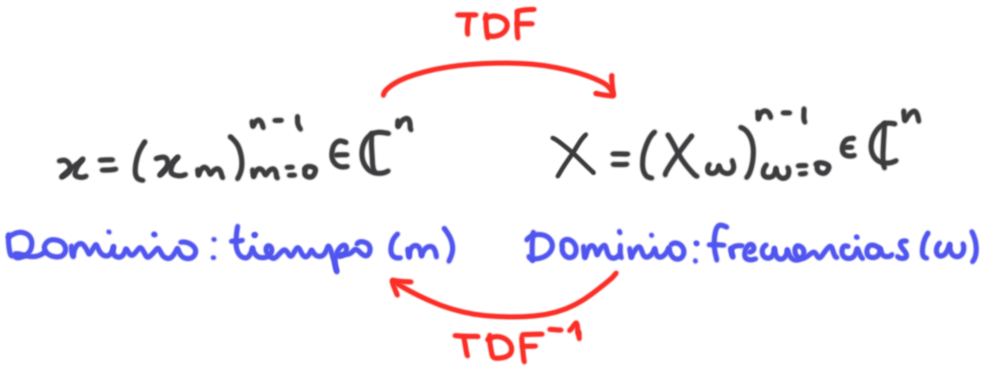
\includegraphics[scale=1.35]{tiempo_freq.png} 
		\caption{Usualmente uno representa a una señal discreta
		$x$ de dimensión $n$ con $n$ mediciones complejas; en este caso, el dominio
		de la representación es el tiempo. Pero
		también se puede representar unívocamente a $x$ con sus
		coeficientes respecto a la base de frecuencias 
		$\cali{B}_{n}$; en este caso, puesto que cada coeficiente da
		el peso que tiene la respectiva frecuencia para construir la 
		señal original $x$, decimos que el dominio de la representación
		es el de frecuencia. Las fórmulas para pasar de una
		representación a otra son \eqref{eq: TDF} y \eqref{eq: TDFI}.}
 	\end{measuredfigure}
\end{figure}


Al usar a $\cali{B}_{n}$ como sistema de representación en
$\IC^{n}$, lo que estamos haciendo es representar a
un $x = (x_{m})_{0 \leq m \leq n-1}$ como combinación
lineal de los vectores 

\[
e_{n,\omega} = \frac{1}{\sqrt{n}} \left( cos
\left( 2 \pi \omega \frac{m}{n} \right)
+ i sen \left( 2 \pi \omega \frac{m}{n}\right) \right)_{0\leq m \leq n-1},
\hspace{0.2cm} 0 \leq \omega \leq n-1;
\]
observe que las partes reales de las
entradas de $e_{n,\omega} \in \IC^{n}$ se obtienen de tomar $n$
muestras uniformes de la función 
$c_{\omega}(t) := \frac{1}{\sqrt{n}} cos (2 \pi \omega t)$ (o sea, de la función
coseno de amplitud $\frac{1}{\sqrt{n}}$, frecuencia $\omega$ y desfase $0$)
y, similarmente,
las partes imaginarias de las entradas se obtienen muestreando
uniformemente a la función 
$s_{\omega}(t) := \frac{1}{\sqrt{n}}  sin (2 \pi \omega t)$.

\begin{figure}[H]
	\sidecaption{
	Por ejemplo, si $n=5$, para construir al vector
	$e_{3}$ de la base $\cali{B}_{n}$ se muestrean uniformemente
	cosenos y senos de frecuencia $3$ como se muestra en la figura;
	los puntos rojos representan las partes reales de las entradas
	y los azules las imaginarias.
	\label{fig: construccion Bn}
	}
	\centering
	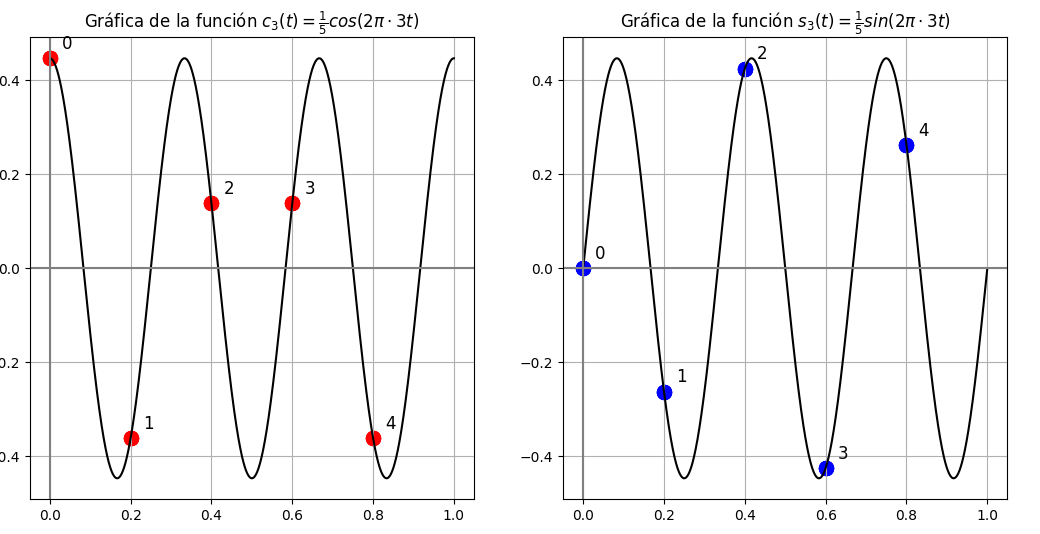
\includegraphics[scale=0.29]{construccion_Bn} 
\end{figure}	

Según esto, el vector $e_{n,\omega}$ se construye a partir
de funciones de frecuencia $\omega$; considerando esto
y el que $\cali{B}_{n}$ sea una BON de $\IC^{n}$ (luego, el
que se valga la identidad de Parseval,
c.f. nota \ref{nota: sobre la identidad de parseval}), tenemos que
la síntesis

\[
x = \suma{\omega=0}{n-1}{\langle x, e_{n,\omega} \rangle e_{n,\omega}}
\]

\noindent
es una expresión de $x$ en términos de vectores de frecuencia
$\omega$ y que los respectivos coeficientes 
$\langle x, e_{n,\omega} \rangle$ indican qué tanto 
contribuye la frecuencia $\omega$ para construir a $x$.

Es por eso que al proceso de considerar representaciones
de señales complejas finitas respecto a las bases de Fourier
se le conoce como  
\textbf{realizar un análisis espectral.}


\subsection{Versión real de la TDF}

En el caso en el que todas las entradas de un vector
$x = (x_{m})_{0 \leq m \leq n-1}$ sean reales, se puede definir
una base ortonormal de $\IR^{n}$, 
análoga a la BON $\cali{B}_{n}$ de $\IC^{n}$ construida en 
\ref{prop: construccion Bn},
a partir de muestreos uniformes
de sinusoides de frecuencias enteras.

\begin{prop}
\label{prop: base de fourier version real}
Sean $n \in \IN$ mayor a uno, $M = \lceil \frac{n}{2} \rceil$.
Definimos a los vectores de $\IR^{n}$

\[
c_{n, 0}= \left( \sqrt{\frac{1}{n}} cos
	\left(2 \pi \cdot 0 \frac{m}{n}
	\right) \right)_{m=0}^{n-1} = 
	\left( \frac{1}{\sqrt{n}}, \cdots, \frac{1}{\sqrt{n}} \right),
\]

	\begin{equation}
	\label{eq0: 10ab}
	c_{n, \omega} := \left( \sqrt{\frac{2}{n}} cos
	\left(2 \pi \omega \frac{m}{n}
	\right) \right)_{m=0}^{n-1},
	\hspace{0.2cm} 1 \leq \omega \leq M-1
	\end{equation}
	
	\begin{equation}
	\label{eq0: 4May}
	s_{n, \omega} := \left( \sqrt{\frac{2}{n}} sin
	\left(2 \pi \omega \frac{m}{n}
	\right) \right)_{m=0}^{n-1},
	\hspace{0.2cm} 1 \leq \omega \leq M-1
	\end{equation}
	
y, en el caso en que n sea par, definimos también
al vector

	\[
c_{n, M}= \left( \sqrt{\frac{1}{n}} cos
	\left(2 \pi \cdot M \frac{m}{n}
	\right) \right)_{0 \leq m \leq n-1} = 
	\left( \frac{(-1)^{m}}{\sqrt{n}} \right)_{m=0}^{n-1}.
\]

El subconjunto $\cali{F}_{n}$ de $\IR^{n}$ definido como

	\begin{itemize}
	\item $\cali{F}_{n} : = \{ c_{n,0}, c_{n,1}, s_{n,1},
	\ldots , c_{n,M-1}, s_{n,M-1}, c_{n,M} \}$ si $n$ es par
	(o sea, si $n=2M$), y como
	\item $\cali{F}_{n} : = \{ c_{n,0}, c_{n,1}, s_{n,1},
	\ldots , c_{n,M-1}, s_{n,M-1} \}$ si $n$ es impar
	(o sea, si $n=2M-1$)
	\end{itemize}
	
es una base ortonormal del $\IR-$espacio vectorial $\IR^{n}$.
\end{prop}

\noindent
\textbf{Demostración.}
Supongamos $n$ par. Si $0 \leq \omega_{1}, \omega_{2} \leq M$
son enteros, entonces
$\omega_{1} + \omega_{2}$ sólo es divisible por $n$ si ambos números
son iguales a $M$. Si suponemos a $\omega_{1}$ y $\omega_{2}$ distintos, 
entonces

\begin{align*}
\langle c_{n, \omega_{1}} , c_{n, \omega_{2}} \rangle = &
\frac{1}{n} \suma{m=0}{n-1}{cos \left(2 \pi \omega_{1} \frac{m}{n} \right) \cdot 
cos \left(2 \pi \omega_{2} \frac{m}{n} \right)} \\
= &\frac{1}{2n} \left(
cos \left(2 \pi (\omega_{1} + \omega_{2}) \frac{m}{n} \right) +
cos \left(2 \pi (\omega_{1} - \omega_{2}) \frac{m}{n} \right)
\right) \\
= & \frac{1}{4n} (
\suma{m=0}{n-1}{
(exp(2 \pi m(\omega_{1}+\omega_{2})i/n) +
exp(-2 \pi m(\omega_{1}+\omega_{2})i) } \\
&  + exp(2 \pi m(\omega_{1}-\omega_{2})i/n) +
exp(-2 \pi m(\omega_{1}-\omega_{2})i)) )\\
\textit{(suma geométrica)} = & 
\frac{exp(2 \pi i (\omega_{1}+\omega_{2}))-1}{4n (exp(2 \pi i (\omega_{1}+\omega_{2})/n)-1)} +
\frac{exp(- 2 \pi i (\omega_{1}+\omega_{2}))-1}{4n (exp(-2 \pi i (\omega_{1}+\omega_{2})/n)-1)}
\\
& + 
\frac{exp(2 \pi i (\omega_{1}-\omega_{2}))-1}{4n (exp(2 \pi i (\omega_{1}-\omega_{2})/n)-1)} +
\frac{exp(- 2 \pi i (\omega_{1}-\omega_{2}))-1}{4n (exp(-2 \pi i (\omega_{1}-\omega_{2})/n)-1)};
\\
\end{align*}

\noindent
puesto que $\omega_{1}+\omega_{2}$ y $\omega_{1}-\omega_{2}$
son ambos enteros, según la proposición 
\ref{prop: propiedades exp compleja} las exponenciales de los numeradores
de esta última expresión son todas iguales a uno, luego, 
$\langle c_{n, \omega_{1}} , c_{n, \omega_{2}} \rangle  =0$. 


Con argumentos similares se prueba 
que todos los elementos de $\cali{F}_{n}$ tienen norma uno, así como
la ortogonalidad entre dos elementos
distintos del conjunto $\cali{F}_{n}$, por lo tanto, la independencia lineal de
este conjunto, luego, el que $\cali{F}_{n}$ sea base 
(ortonormal) de $\IR^{n}$.


\QEDB
\vspace{0.2cm}



\begin{defi}
Sea $n \in \IN$, $n \geq 2$. Llamaremos a la BON
$\cali{F}_{n}$ de $\IR^{n}$ definida en \ref{prop: base de fourier version real}
la \textbf{base de Fourier real de dimensión $n$}.
\end{defi}

\begin{nota}
\label{nota: frecuencias en las bases de fourier}
Observe que $\cali{F}_{n}$, a diferencia de $\cali{B}_{n} \subseteq \IC^{n}$, 
considera frecuencias enteras no mayores a $M := \lceil \frac{n}{2} \rceil$
(cuando $n$ es par) o a $M-1$ (cuando $n$ es impar), mientras que
en $\cali{B}_{n}$ se consideran las frecuencias enteras entre $0$
y $n-1$ (inclusivo); así, si decidimos representar
a una señal $x \in \IR^{n}$ en base a $\cali{F}_{n} \subseteq \IR^{n}$
y no en base a $\cali{B}_{n} \subseteq \IC^{n}$, sintetizaremos a $x$
respecto a frecuencias enteras acotadas por $M$ o por $M-1$ 
(dependiendo de la paridad de $n$), y no respecto a frecuencias
menores a $n$.
\end{nota}

\begin{ejemplo}
\label{ej: DFT1}
Consideremos a la señal 
\begin{equation}
\label{eq2: 10ab}
x=(-0.5,-8,-5.3,15,-0.3,6,4) \in \IR^{7}.
\end{equation}

Según la construcción de $\cali{F}_{7}$ (c.f. 
proposición \ref{prop: base de fourier version real}),
una expresión de $x$ respecto a $\cali{F}_{7}$ 
es una síntesis de $x$ a partir de señales 
de frecuencias $\omega = 0,1,2,3$. En la imagen de abajo
se muestran los coeficientes de $x$ respecto a $\cali{F}_{7}$.

\begin{figure}[H]
	\sidecaption{
	Se muestran la gráfica de $x$ junto con la gráfica de los
	coeficientes de $x$ respecto a la BON $\cali{F}_{7}$. Observe 
	que, por definición, sólo un vector de $\cali{F}_{7}$ tiene frecuencia
	cero (i.e. es constante), mientras que para las otras frecuencias
	tenemos dos vectores de la misma frecuencia, uno construido a partir de un 			
	coseno y otro a partir de un seno.
	\label{fig: ejFrecuencia 1}
	}
	\centering
	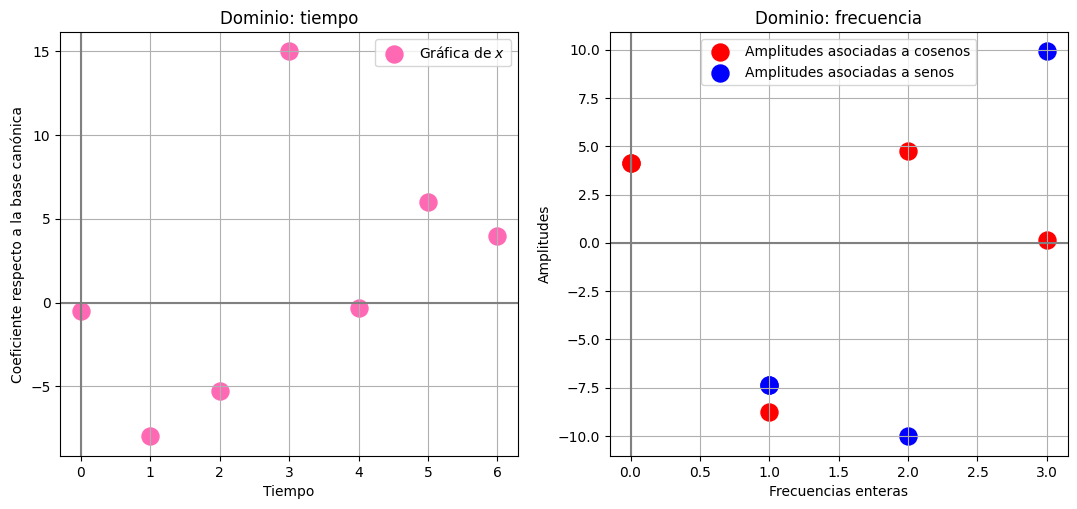
\includegraphics[scale=0.4]{ejFrecuencia_1} 
\end{figure}	

Redondeando los coeficientes, 
se tiene la siguiente descomposición de $x$;

\begin{equation}
\label{eq: analisis x TDF}
x = 4.12 c_{7,0} - 8.76c_{7,1} -7.35s_{7,1}+
4.77c_{7,2}-10s_{7,2}+0.14c_{7,3}+9.91s_{7,3}.
\end{equation}

\noindent
A continuación mostramos las gráficas
de los sinusoides que fueron discretizados
para obtener los vectores de frecuencia
$0,1,2$ y $3$ en los que descompusimos a $x$.

\begin{figure}[H]
	\sidecaption{
	Aporte de frecuencia $0$.
	\label{fig: ejFrecuencia 2}
	}
	\centering
	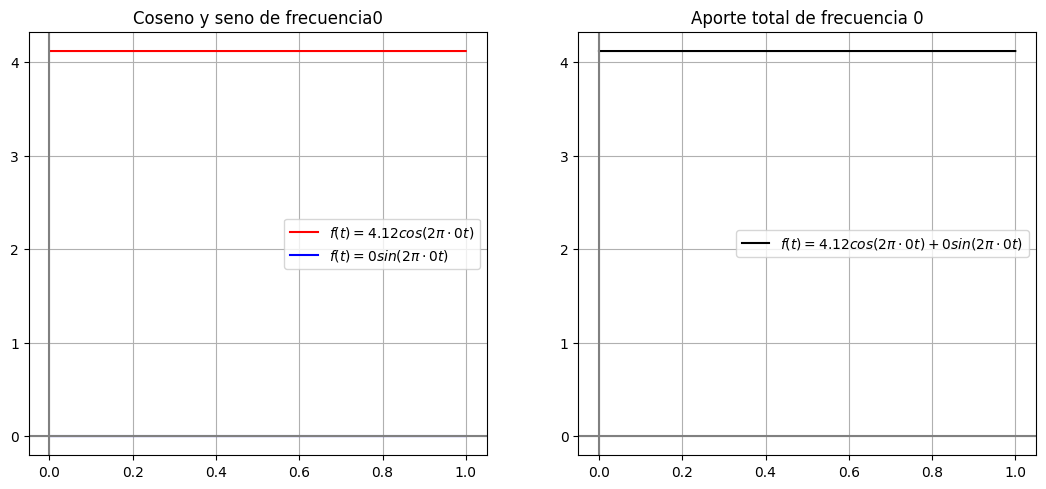
\includegraphics[scale=0.4]{ejFrecuencia_2} 
\end{figure}	

\begin{figure}[H]
	\sidecaption{
	Aporte de frecuencia $1$.
	\label{fig: ejFrecuencia 3}
	}
	\centering
	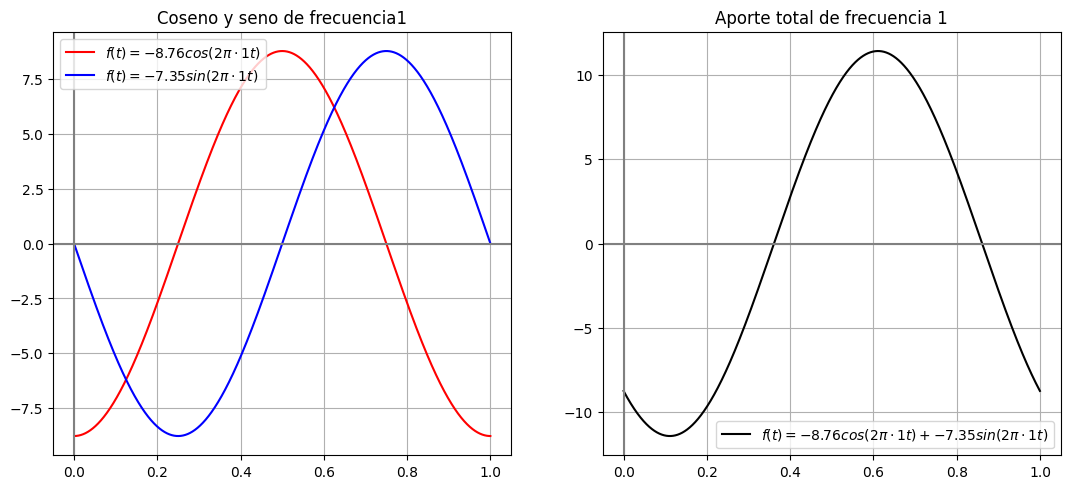
\includegraphics[scale=0.4]{ejFrecuencia_3} 
\end{figure}	

\begin{figure}[H]
	\sidecaption{
	Aporte de frecuencia $2$.
	\label{fig: ejFrecuencia 4}
	}
	\centering
	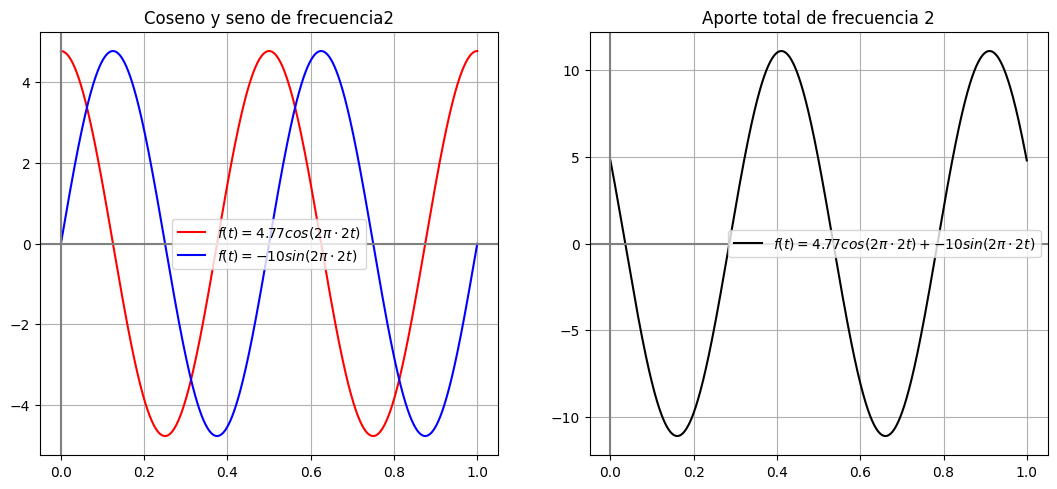
\includegraphics[scale=0.4]{ejFrecuencia_4} 
\end{figure}	


\begin{figure}[H]
	\sidecaption{
	Aporte de frecuencia $3$.
	\label{fig: ejFrecuencia 5}
	}
	\centering
	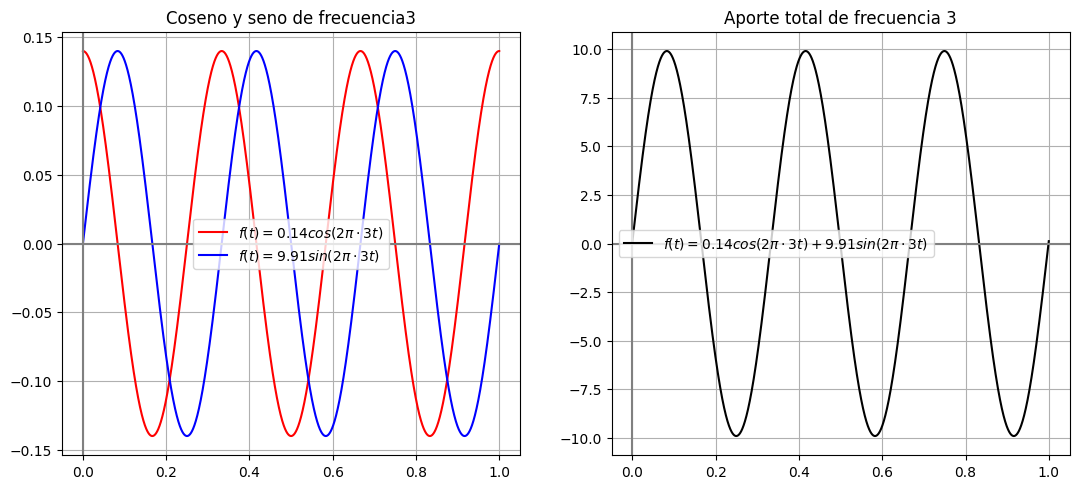
\includegraphics[scale=0.4]{ejFrecuencia_5} 
\end{figure}	

Sumando todas las gráficas de la derecha, obviamente
obtenemos una función de cosenos y senos tal que,
del muestrearla uniformemente en $[0,1]$, resulta
el vector $x$ \eqref{eq2: 10ab}.

\begin{figure}[H]
	\sidecaption{
	En morado se muestra la gráfica de la función suma
	de las gráficas derechas en las figuras anteriores.
	\label{fig: ejFrecuencia 6}
	}
	\centering
	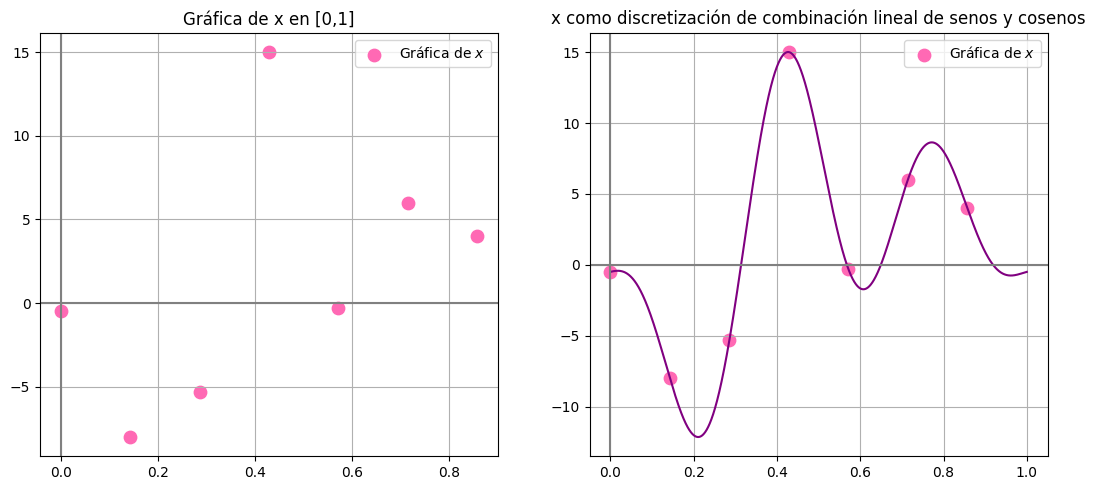
\includegraphics[scale=0.44]{ejFrecuencia_6} 
\end{figure}	
\final
\end{ejemplo}

Para terminar, digamos en concreto qué se entiende
por el espectro que resulta de usar la 
versión real de la transformada
discreta de fourier para analizar una señal finita.

En la definición 
$\cali{F}_{n}$ de la base dada en 
\ref{prop: base de fourier version real}, observe que, 
por cada frecuencia entera $\omega$ considerada,
aparecen uno o dos sinusoides (discretizados) con tal frecuencia:


\begin{table}[ht]
\sidecaption{Dimensión $n = 2M-1$ impar}
\centering
  \begin{tabular}{ l | c | c | c | c }
    \hline
    Frecuencia & $0$ & $1$ & $\ldots$ & $M-1$  \\ \hline
    Cant. sinusoides  & $1$ & $2$ & $\ldots$ & $2$ \\
    \hline
  \end{tabular}
\label{Tab: frecuencias TDF n impar}
\end{table}

\vspace{2cm}

\begin{table}[ht]
\sidecaption{Dimensión $n = 2M$ par}
\centering
  \begin{tabular}{ l | c | c | c | c | c}
    \hline
    Frecuencia & $0$ & $1$ & $\ldots$ & $M-1$ & $M$  \\ \hline
    Cant. sinusoides  & $1$ & $2$ & $\ldots$ & $2$ & $1$ \\
    \hline
  \end{tabular}
\label{Tab: frecuencias TDF n par}
\end{table}

\begin{defi}
\label{def. Dom tdf}
Sea $n \geq 2$. Llamaremos $Dom_{TDF, n}$ al conjunto de frecuencias
consideradas en la transformada discreta de Fourier para
las señales de dimensión $n$, o sea, al siguiente subconjunto de $\IR$;

\[
Dom_{TDF, n} = \{ 0 , 1, \cdots, M-1 \}
\hspace{0.2cm} \text{si } n = 2M-1
\hspace{0.2cm}
\text{es impar, }
\]
y
\[
Dom_{TDF, n} = \{ 0 , 1, \cdots, M \}
\hspace{0.2cm} \text{si } n = 2M-1
\hspace{0.2cm}
\text{es par.}
\]
\end{defi}


\begin{nota}
\label{nota: ya?}
Por ser 
la base de Fourier real
$\cali{F}_{n}$ una BON de $\IR^{n}$, 
si $M = \lceil \frac{n}{2} \rceil$,
\begin{equation}
\label{ec: sintesis 0}
x = \langle x , c_{n, 0} \rangle c_{n, 0} + \suma{\omega = 1}{M-1}{(
\langle x , c_{n, \omega} \rangle c_{n, \omega} + 
\langle x , s_{n, \omega} \rangle s_{n, \omega} )}
\hspace{0.2cm} \text{si n es impar}
\end{equation}

\begin{equation}
\label{ec: sintesis 1}
x = \langle x , c_{n, 0} \rangle c_{n, 0} + \suma{\omega = 1}{M-1}{(
\langle x , c_{n, \omega} \rangle  c_{n, \omega} + \langle x , s_{n, \omega} \rangle
s_{n, \omega} )}
+ \langle x , c_{n, M} \rangle c_{n, M} 
\hspace{0.2cm} \text{si n es par;}
\end{equation}

así, usando la transformada discreta de Fourier
-que, en este contexto, pensamos como calcular
los coeficientes de $x$ respecto a $\cali{F}_{n}$- 
tenemos tanto
un proceso de análisis de $x$ (que pensamos como
el cálculo de tales coeficientes)
respecto a sinusoides discretizados
de frecuencias $\omega \in Dom_{TDF, n}$
como uno de síntesis, que interpretamos como
el recuperar a la señal original $x$ usando
sus coeficientes respecto a $\cali{F}_{n}$.
\end{nota}

Se vale además la
identidad de Parseval, luego, para toda
señal $x \in \IR^{n}$,

\begin{equation}
\label{eq0: 25Ap}
||x||^{2} = \langle x , c_{n,0} \rangle^{2}+
\suma{\omega=0}{M-1}{(\langle x , c_{n,\omega} \rangle^{2} + 
\langle x , s_{n,\omega} \rangle^{2})}
\hspace{0.2cm} \textit{si n es impar} 
\end{equation}
y
\begin{equation}
\label{eq1: 25Ap}
||x||^{2} = \langle x , c_{n,0} \rangle^{2}+
\suma{\omega=0}{M-1}{(\langle x , c_{n,\omega} \rangle^{2} + 
\langle x , s_{n,\omega} \rangle^{2})}
+ \langle x , c_{n,M} \rangle^{2}
\hspace{0.2cm} \textit{si n es par};
\end{equation}
así, los coeficientes de la forma
$\langle x , c_{n,\omega} \rangle^{2}$ y 
$\langle x , s_{n,\omega} \rangle^{2}$
dan información sobre el peso que la frecuencia
$\omega$ tiene para sintetizar a la señal $x$.

\marginnote{Según las ecuaciones \eqref{eq0: 25Ap}
y \eqref{eq1: 25Ap}, los coeficientes $\tau_{n, \omega}(x)$
permiten calibrar la presencia de la frecuencia $\omega$
(en los rangos dados por las tablas 6.1 y 6.2)
en una señal $x$.}

\begin{defi}
\label{def: taus}
Sean $n \geq 2$, $M = \lceil \frac{n}{2} \rceil $.
Definimos
	\[
	\tau_{n}(x, 0) := \frac{|\langle x, c_{n,0} \rangle|}{|| x ||} ,	
	\]
	y
	\[
	\forall 
	\hspace{0.1cm}	
	1 \leq \omega \leq M-1: \hspace{0.2cm} 
	\tau_{n}(x, \omega) := 
	\frac{\sqrt{
	\langle x, c_{n,\omega} \rangle^{2}+
	\langle x, s_{n,\omega} \rangle^{2}}}{||x||}.	
	\]	
		Si $n$ es par, se define además a
	\[
	\tau_{n}(x, M) := 
	\frac{ |\langle x, c_{n,M} \rangle| }{ ||x|| }.
	\]
\end{defi}
De las ecuaciones 
\eqref{eq0: 25Ap} y 
\eqref{eq1: 25Ap} se deduce
fácilmente que, para toda $\omega$, 
$0 \leq \tau_{n}(x, \omega) \leq 1$. Puede pensar
a tales coeficientes $\tau_{n}(x, \omega)$ como la
contribución (normalizada por la norma de $x$)
de la frecuencia $\omega$ para sintetizar a $x$.


\begin{defi}
\label{def: espectro DFT}
Sean $n \geq 2$,  $x \in \IR^{n}$. Por el 
\textbf{espectro de $x$ 
obtenido a partir de la TDF} nos referiremos
a la 
función 
$\mathrm{T}_{x} : Dom_{TDF, n} \longrightarrow [0, 1] \subseteq \IR$
definida como
\[
\mathrm{T}_{x} (\omega) = \tau_{n}(x, \omega)
\hspace{0.2cm} \text{ para toda }
\hspace{0.2cm} \omega \in Dom_{TDF, n},
\]
donde los coeficientes $\tau_{n}(x, \omega)$
son como se definieron en \ref{def: taus}
\end{defi}

\begin{ejemplo}
A continuación se grafica el espectro
(a la derecha) obtenido
a partir de la TDF de la señal considerada en el 
ejemplo \ref{ej: DFT1}.

\begin{figure}[H]
	\sidecaption{
	Espectro de la señal $x$ dada en 
	\eqref{eq2: 10ab}. 
	\label{fig: dft_espectro_1}
	}
	\centering
	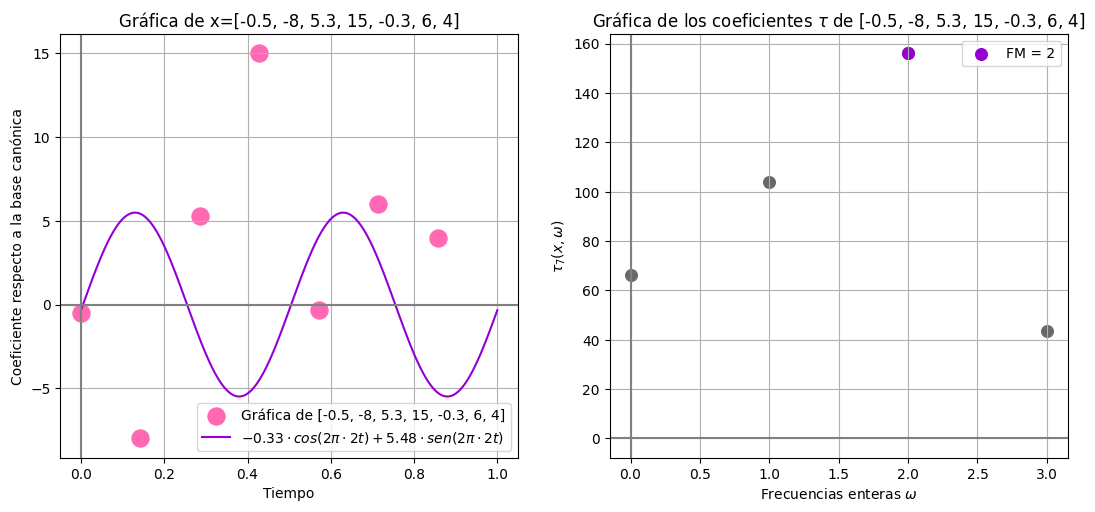
\includegraphics[scale = 0.45]{dft_espectro_1} 
\end{figure}	

Como se marca en el espectro con color morado, la frecuencia
asociada al coeficiente $\tau$ más alto es $\omega =2$; a la
izquierda, junto con la gráfica de la señal 
$x$, se dibuja el sinusoide (en versión continua)
de frecuencia $2$ que aparece en el análisis de
$x$ respecto a $\cali{F}_{7}$ dado en 
\eqref{eq: analisis x TDF}.
\final
\end{ejemplo}
\section{Caso particular en el que el subespacio en cuestión es un plano}
\label{ap: Caso particular en el que el subespacio en cuestión es un plano}

\TODO{Cambiar título e intro porque moví esto.}
Necesitaremos concentrarnos en el caso
particular en el que el subespacio cerrado $W$ es 
un plano,\sidenote{O sea, un subespacio
de dimensión $2$.} por lo que a continuación elaboramos un poco más
la teoría de la sección 
\ref{angulo entre elementos de un espacio con producto punto}
para este caso particular.

La situación es la siguiente: $V$ es un $\IR-$espacio
de Hilbert, $u$ y $v$ son elementos de $V$,
unitarios y linealmente
independientes entre sí. El espacio que ellos generan
es pues un plano, digamos,


\[
P := span \{ u, v \}.
\]

Dado $x \in V$,
el coseno del ángulo entre $x$ y $W$ es,
según la proposición
\ref{prop: algunos hechos sobre el angulo entre un vector y un subespacio},

\begin{equation}
\label{eq0: 19Marzo}
cos \left( \measuredangle (x, P) \right) = 
\frac{|| \Pi_{P}(x) ||}{||x||};
\end{equation}
para lograr expresar el lado derecho de la igualdad en términos
sólo de $u$, $v$ y $x$ (que son los elementos básicos de
nuestra discusión), conviene primero obtener, a partir 
de estos elementos, una base
ortonormal del espacio $P$.


\begin{obs}
Si $u, v \in V$ son unitarios y linealmente independientes, y $P$
es el plano que generan, entonces
$\{ u, z \}$, donde

\begin{equation}
\label{eq2: 19Marzo}
z:= \frac{v- \langle u, v \rangle u}{||v- \langle u, v \rangle u||}
\end{equation}
es una BON de $P$
\end{obs}
\noindent
\textbf{Demostración.}
Basta aplicar el teorema de Gram-Schmidt 
\ref{Teo:Gram-Schmidt}.
\QEDB
\vspace{0.2cm}

Teniendo una BON de $P$, según el 
corolario 
\ref{cor: proyeccion en terminos de BON}, se tiene la siguiente
expresión para la proyección de $x$ en $P$;

\begin{equation}
\label{eq1: 19Marzo}
\Pi_{P}(x)= \langle x, u \rangle u + \langle x, z \rangle z;
\end{equation}

\noindent
puesto que, según la definición \eqref{eq2: 19Marzo} de 
$z$ este vector es función de $u$ y $v$, fácilmente se
puede derivar, a partir de \eqref{eq1: 19Marzo},
una expresión de $\Pi_{P}(x)$ en función sólo
de $x$, $u$ y $v$. Se plasman las fórmulas 
concretas a continuación.
	\begin{prop}
	\label{prop: formulas 20Marzo}
	Sean $V$ un espacio de Hilbert, $x \in V$,
	$u,v \in V$ linealmente independientes
	y unitarios. Si $P$ es el plano
	que generan $u$ y $v$, entonces,

		\begin{equation}
		\label{eq0: 24ap}
		\Pi_{P}(x)= \frac{\langle x, u \rangle -\langle u, v \rangle \langle x, v \rangle }{1-\langle u, v \rangle^{2}} u + \frac{\langle x, v \rangle -\langle u, v \rangle \langle x, u \rangle }{1-\langle u, v \rangle^{2}} v
		\end{equation}
	y 
		\begin{equation}
		\label{eq3: 19Marzo}
		  || \Pi_{P}(x) ||^{2}=
		  \frac{\langle x, u \rangle^{2} +  \langle x, v \rangle^{2}	
	       -2  \langle x, u \rangle \langle x, v \rangle \langle u, v \rangle	}{1- \langle u, v 		\rangle^{2}}.
		\end{equation}
 
	\end{prop}

\noindent
\textbf{Demostración.}
La demostración consiste de simples manipulaciones aritméticas.
Según \eqref{eq1: 19Marzo},
\begin{align*}
\Pi_{P}(x) = & \langle x, u \rangle u + \langle x, z \rangle z \\
 = & \langle x, u \rangle u
 + \frac{\langle x, v \rangle - \langle u, v \rangle \langle x, u \rangle}{|| v -\langle u,v \rangle u ||^{2}}
(v - \langle u,v \rangle u);\\
\end{align*}

\noindent
puesto que $u$ y $v$ son unitarios, 
tenemos que
\begin{align}
\label{eq3: 23ap}
|| v -\langle u,v \rangle u ||^{2} = & 
\langle v,v \rangle^{2} -2
\langle u,v \rangle^{2} +\langle u,v \rangle^{2}\langle u,u \rangle \notag  \\
= & 1 -\langle u,v \rangle^{2}; 
\end{align}
sustituyendo \eqref{eq3: 23ap} en la última expresión para 
$\Pi_{P}(x)$ llegamos a \eqref{eq3: 19Marzo}. \\

Finalmente, 
\begin{align*}
|| \Pi_{P}(x) ||^{2} = & 
\langle x,u \rangle^{2} + \langle x,z \rangle^{2} \\
= & \langle x,u \rangle^{2} + 
\left(
\frac{\langle x,v \rangle - \langle u,v \rangle
\langle x,u \rangle}{||v -\langle u,v \rangle u ||}
\right)^{2};\\
\end{align*}

\noindent
sustituyendo \eqref{eq3: 23ap} en esta última expresión
llegamos a \eqref{eq4: 19Marzo}.

\QEDB
\vspace{0.2cm}

Usando las expresiones
\eqref{eq: coseno a subespacio}
y \eqref{eq3: 19Marzo} es fácil establecer
la siguiente proposición.

\begin{prop}
Sean $V$ un espacio de Hilbert, $x \in V$,
	$u,v \in V$ linealmente independientes
	y unitarios. Si $P$ es el plano
	que generan $u$ y $v$, entonces,
	
	
\begin{equation}
\label{eq: coseno a plano}
cos (\measuredangle (x, P)) = 
\sqrt{
\frac{\langle x, u \rangle^{2} +  \langle x, v \rangle^{2}	
	       -2  \langle x, u \rangle \langle x, v \rangle \langle u, v \rangle	}{
	       ||x||^{2} \cdot 
	       (1- \langle u, v 	\rangle^{2})  }}.
\end{equation}
\end{prop}


\section{Metodología para realizar un análisis espectral que considere frecuencias arbitrarias}
\label{sec: metodologia para realizar un analisis espectral que considere frecuencias arbitrarias}

Ya podemos usar la base de Fourier real $\cali{F}_{n}$
definida en la proposición \ref{prop: base de fourier version real}
para hacer un estudio espectral de los PDL. \TODO{Grafico
algunos resultados en otro capítulo?} \\


Puesto que, por la construcción de $\cali{F}_{n}$, 
hacer un análisis espectral de una señal $x \in \IR^{n}$
via su análisis respecto a la BON $\cali{F}_{n}$ nos lleva
a considerar sólo ciertas frecuencias enteras
(c.f. nota \ref{nota: frecuencias en las bases de fourier}),
queremos no sólo usar la TDF para realizar
nuestro estudio espectral, pues
no queremos restringirnos
al estudio de frecuencias enteras
(después de todo, según la hipótesis planteada en 
\ref{ref: hipotesis}, 
creemos que la frecuencia que mejor aproxima al PDL
$\cali{L}^{n,k}$ es $\frac{k}{2}$, y este último número no siempre
es un entero), sino que nos gustaría
\begin{enumerate}
	\item poder elegir una frecuencia $\omega \geq 0$ respecto
a la cual comparar a la señal y,
	\item una vez fijada una frecuencia, buscar el desfase $\phi \in [0,1]$
	que mejor ajuste la gráfica de $x$.
\end{enumerate}

\begin{figure}[H]
	\sidecaption{
	Aquí se grafica una misma señal $x \in \IR^{16}$ y se 
	compara con dos sinusoides de frecuencia $3.6$, una con 
	desfase (normalizado) 0.8 y otra con 0.32. Observe que
	la primera parece ajustar mucho mejor la gráfica de $x$.
	\label{fig: ejemplo desfase}
	}
	\centering
	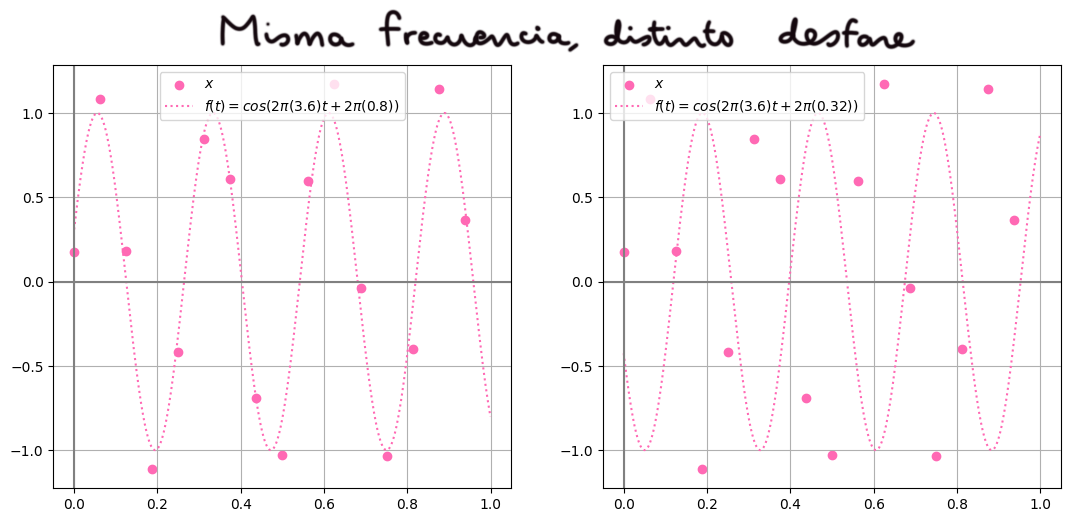
\includegraphics[scale=0.45]{desfase_ejemplo} 
\end{figure}	


Vamos a seguir
una linea de razonamiento totalmente análoga a la empleada 
en el ejemplo \ref{subs: ejm 3}, pues aquí también abordamos el problema
definiendo cúmulos
\sidenote{Hablamos más precisamente
de subespacios de $\IR^{n}$, pero 
\TODO{notación de DS. Habla tamién de esto 
en el ap. de cosine sim.}}
de $\IR^{n}$ que consten de elementos que cumplan
determinada propiedad (en el caso del ejemplo \ref{subs: ejm 3}, la propiedad
era ser elemento de determinado espacio $W_{n,k}$ mientras que 
en esta sección la propiedad de nuestro interés es ``ser la discretización
de un sinusoide de frecuencia $\omega$'') y usando el coseno del ángulo que
una señal $x$ forma con dichos cúmulos para dar una medida de qué tanto
tiene $x$ la propiedad considerada.


usamos el coseno del ángulo que forma una señal $x \in \IR^{n}$
con el plano $W_{n,1}$ para dar una medida de qué tan afín es $x$;
queremos ahora hacer algo similar, y usar el coseno de $x$ con espacios
de frecuencias $\omega >0$ como
una medida de qué tanto reacciona $x$ a la frecuencia $\omega$.



\begin{notacion}
Para simplificar la notación, denotamos por $I_{n}$ al intervalo
$\{ \frac{m}{n}  : 0 \leq m \leq n-1 \}$.
\end{notacion}

Digamos qué es lo que 
entendemos por ``señal de frecuencia pura $\omega$''.

\begin{defi}
Sean $n \in \IN$,  $\omega>0$, $\phi \in [0,1[$.  
A toda señal $n-$dimensional  
de la forma

\begin{equation}
A \left(
cos \left(  2 \pi \omega t + 2 \pi \phi
\right)
\right)_{t \in I_{n}}
\end{equation}

\noindent
con $A \in \IR$, se le llamará
\textbf{señal $n-$dimensional de frecuencia
pura $\omega$}. En este contexto,
a $\phi$ se le llama el \textbf{desfase normalizado}
de la señal, y a $A$ la \textbf{amplitud}.
\end{defi}

\begin{nota}
Observe que toda señal de la forma
\begin{equation*}
A \left(
sin \left(  2 \pi \omega t + 2 \pi \phi
\right)
\right)_{t \in I_{n}},
\end{equation*}
con $A \in \IR$, también es una señal $n-$dimensional
de frecuencia pura $\omega$, pues, como 
\[
sen(x) = - cos (x+ \pi/2) \hspace{0.2cm}
\textit{para toda } x \in \IR,
\]
entonces
\begin{equation*}
A \left(
sin \left(  2 \pi \omega t + 2 \pi \phi
\right)
\right)_{t \in I_{n}} =
-A \left(
cos \left(  2 \pi \omega t + 2 \pi \phi^{'}
\right)
\right)_{t \in I_{n}},
\end{equation*}
donde $\phi^{'}= (\phi + 1/4) \% 1 \in [0,1[$.
\end{nota}


\begin{figure}[H]
	\sidecaption{
	Se grafica a la función 
	$f(t) = cos(2 \pi \cdot \frac{5}{2} t + 2 \pi \cdot 0.3)$;
	muestreando este sinusoide de forma uniforme en el 
	intervalo [0,1] obtenemos una señal de frecuencia pura
	$\omega = \frac{5}{2}$. En la figura, $n=5$.
	\label{fig: muestreo coseno}
	}
	\centering
	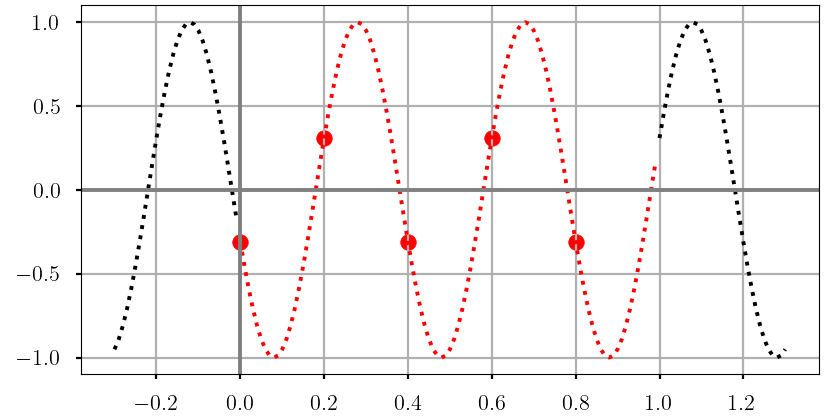
\includegraphics[scale= 0.55]{muestreo_coseno} 
\end{figure}	

\begin{prop}
\label{prop: para que frecuencias omega vector seno es cero}
	Sean $n \geq 2$, $\omega \geq 0$.
	\begin{itemize}
		\item El vector 
		\begin{equation}
		\label{eq: coseno omega}
		c_{n, \omega} = \left(cos(2 \pi \omega m/n) \right)_{m=0}^{n-1} \in \IR^{n}
		\end{equation}
		no es cero, y 
		\item el vector 
		\begin{equation}
		\label{eq: seno omega}
		s_{n, \omega} = \left(sen(2 \pi \omega m/n) \right)_{m=0}^{n-1} \in \IR^{n}
		\end{equation}
		es cero si y sólo si $\omega \in \frac{n}{2} \IZ$.
	\end{itemize}
\end{prop}
\noindent
\textbf{Demostración.}
El primer punto es fácil de probar, pues la primera entrada del
vector \eqref{eq: coseno omega} es 
$cos(0)=1$.

Supogamos ahora que $\omega>0$ es tal que \eqref{eq: seno omega}
es el vector cero, o sea, que
para toda $0 \leq m \leq n-1$, se tiene que 
$sen(2 \pi \omega m/n)=0$. En particular, ocurre
$sen(2 \pi \omega /n)=0$; esto implica la igualdad 
$2 \pi \omega /n = \pi K$ para algún entero $K$. Despejando
a $\omega$ de la ecuación tenemos que 
$\omega = \frac{n}{2}K \in \frac{n}{2} \IZ$. Recíprocamente,
todo $\omega$ de la forma 
$\frac{n}{2}K$, con $K \in \IZ$ hace que el vector 
\eqref{eq: seno omega} sea cero, pues, para toda $0 \leq m \leq n-1$,
$sen\left(2 \pi \frac{n}{2}K \frac{m}{n}\right)=
sen((Km)\pi)=0$.
\QEDB
\vspace{0.2cm}


\begin{obs}
\label{obs: f y g son l.i. y de norma uno}
Sean $n \geq 2$ entero, $\omega \geq 0$ con $\omega \not\in \frac{n}{2} \IZ$.
Los vectores \eqref{eq: coseno omega} y \eqref{eq: seno omega}
de $\IR^{n}$ son linealmente independientes.
\end{obs}
\noindent
\textbf{Demostración.}
Sólo note que 
la primera entrada de \eqref{eq: coseno omega} es $1$, mientras que  
la primera entrada de $g_{n, \omega}$ sea cero, pero no
todas sus entradas sean cero (c.f. proposición 
\ref{prop: para que frecuencias omega vector seno es cero}). 
\QEDB
\vspace{0.2cm}


Según la observación 
\ref{obs: f y g son l.i. y de norma uno}, si $\omega \not\in \frac{n}{2} \IZ$,
el espacio $P_{n,\omega}$ que generan los vectores 
\eqref{eq: coseno omega} y \eqref{eq: seno omega}

\begin{align}
\label{eq6: 23Ap}
P_{n,\omega}:= & span(c_{n, \omega}, s_{n, \omega}) \notag  \\  
= &
\{ a \left( cos \left(2 \pi \omega t \right) \right)_{t \in I_{n}} +
b ( sen (2 \pi \omega t ))_{t \in I_{n}} : 
\hspace{0.2cm} a, b \in \IR \},
\hspace{0.1cm} \omega \not\in \frac{n}{2} \IZ
\end{align}

\noindent
es un plano (i.e. un subespacio de dimensión $2$) de $\IR^{n}$.
\begin{prop}
\label{prop: Pw consta de las señales de frecuencia omega}
Sean $n \in \IN$, $\omega \geq 0$ 
con 
$\omega \not\in \frac{n}{2} \IZ$.
El espacio $P_{n, \omega}$ definido en \eqref{eq2: 20Marzo} consta exactamente
de las señales $n$ dimensionales de frecuencia $\omega$.
\end{prop}

\noindent
\textbf{Demostración.}

Sea $\phi \in [0,1]$ un desfase cualquiera y $A \in \IR$
una amplitud cualquiera; por la regla
del coseno de la suma de dos ángulos, tenemos que
\[
A(cos (2 \pi \omega t + 2 \pi \phi))_{t \in I_{n}}
= Aa  (cos(2 \pi \omega t))_{t \in I_{n}} +
Ab  (sen(2 \pi \omega t))_{t \in I_{n}} \in P_{\omega} \in P_{\omega}
\]
donde
\[
a := cos (2 \pi \phi) \hspace{0.2cm} \text{y}
\hspace{0.2cm} b := sin (2 \pi  \phi).
\]


Recíprocamente, si $a, b \in \IR$ son escalares cualesquiera, 
el elemento genérico
$x=  a \left( cos \left(2 \pi \omega t \right) \right)_{t \in I_{n}} +
b ( sen (2 \pi \omega t ))_{t \in I_{n}} $ de $P_{n,w}$ puede
expresarse como sigue:

\begin{equation}
\label{eq1: 28Mar23}
x = \sqrt{a^{2}+b^{2}} \left(
A  \left( cos \left(2 \pi \omega t \right) \right)_{t \in I_{n}} +
B  \left( sin \left(2 \pi \omega t \right) \right)_{t \in I_{n}}
\right),
\end{equation}

\noindent
donde
\[
A := \frac{a}{\sqrt{a^{2}+b^{2}}} \hspace{0.2cm} \text{y} \hspace{0.2cm}
B := \frac{b}{\sqrt{a^{2}+b^{2}}}.
\]
Como $A^{2}+ B^{2}=1$, existe $\phi \in [0,1]$ tal que
\begin{equation}
\label{eq0: 28Mar23}
A = cos (2 \pi \phi) \hspace{0.2cm} \text{y}  \hspace{0.2cm}
B = sin (2 \pi \phi);
\end{equation}
sustituyendo \eqref{eq0: 28Mar23} en \eqref{eq1: 28Mar23}, llegamos
a que

\begin{align*}
x = &  \sqrt{a^{2}+b^{2}} (
cos(2 \pi \phi) \cdot (cos (2 \pi \omega t))_{t \in I_{n}} + 
sin(2 \pi \phi) \cdot (sin (2 \pi \omega t))_{t \in I_{n}} 
) \\
= & \sqrt{a^{2}+b^{2}} (
cos(2 \pi \phi) \cdot cos (2 \pi \omega t) +
sin(2 \pi \phi) \cdot sin (2 \pi \omega t) 
)_{t \in I_{n}}  \\
= &  \sqrt{a^{2}+b^{2}} (
cos (2 \pi \omega t - 2 \pi \phi)
)_{t \in I_{n}}.
\end{align*}

\QEDB
\vspace{0.2cm}


\noindent 
Según la proposición
\ref{prop: Pw consta de las señales de frecuencia omega},
$P_{n, \omega} \subseteq \IR^{n}$ es el plano que consiste de las señales
de dimensión $n$ y frecuencia (pura) $\omega$.

Si $\omega \in \frac{n}{2} \IZ$, entonces, según 
la proposición 
\ref{prop: para que frecuencias omega vector seno es cero}, el vector
$s_{n, \omega}$ es el vector cero y $c_{n, \omega}$, luego, el espacio
\begin{align}
\label{eq0: 23Ap}
P_{n,\omega}:= & span(c_{n, \omega}, s_{n, \omega}) \notag  \\  
= &
\{ a \left( cos \left(2 \pi \omega t \right) \right)_{t \in I_{n}} : 
\hspace{0.2cm} a \in \IR \},
\hspace{0.1cm} \omega \in \frac{n}{2} \IZ
\end{align}
es una recta (i.e. un subespacio de dimensión $1$)
de $\IR^{n}$.

\begin{defi}
Si $n \geq 2$ y $\omega>0$, entonces
al subespacio $P_{n,\omega}$ 
de $\IR^{n}$,
definido en \eqref{eq2: 20Marzo} si 
$\omega \not\in \frac{n}{2} \IZ$ y en 
\eqref{eq0: 23Ap} en caso contrario,
le llamaremos el \textbf{espacio monofrecuencial
$n$ dimensional} de frecuencia $\omega$.
\end{defi}


Es razonable pues
medir la cercanía de una señal $n-$dimensional $x \in \IR^{n}$
a tener frecuencia $\omega$
con el ángulo que $x$ forma con el subespacio $P_{n, \omega}$,
cuyo coseno, según la proposición
\ref{prop: algunos hechos sobre el angulo entre un vector y un subespacio}
es
\begin{equation}
\label{eq0: 20Mar}
cos \left( \measuredangle (x, W) \right) = \frac{|| \Pi_{W}(x) ||}{||x||}
\in [0,1].
\end{equation}


\begin{figure}[H]
	\sidecaption{
	Según la relación \eqref{eq0: 20Mar}, 
	si $\frac{||\Pi_{P_{\omega}}(x)||}{||x||}$ es cercano 
	a uno (resp. a cero), entonces $x$ es muy parecido a una señal de frecuencia $\omega$
	(resp. se aleja de ser una señal de frecuencia $\omega$).
	\label{fig: 20Mar23_1}
	}
	\centering
	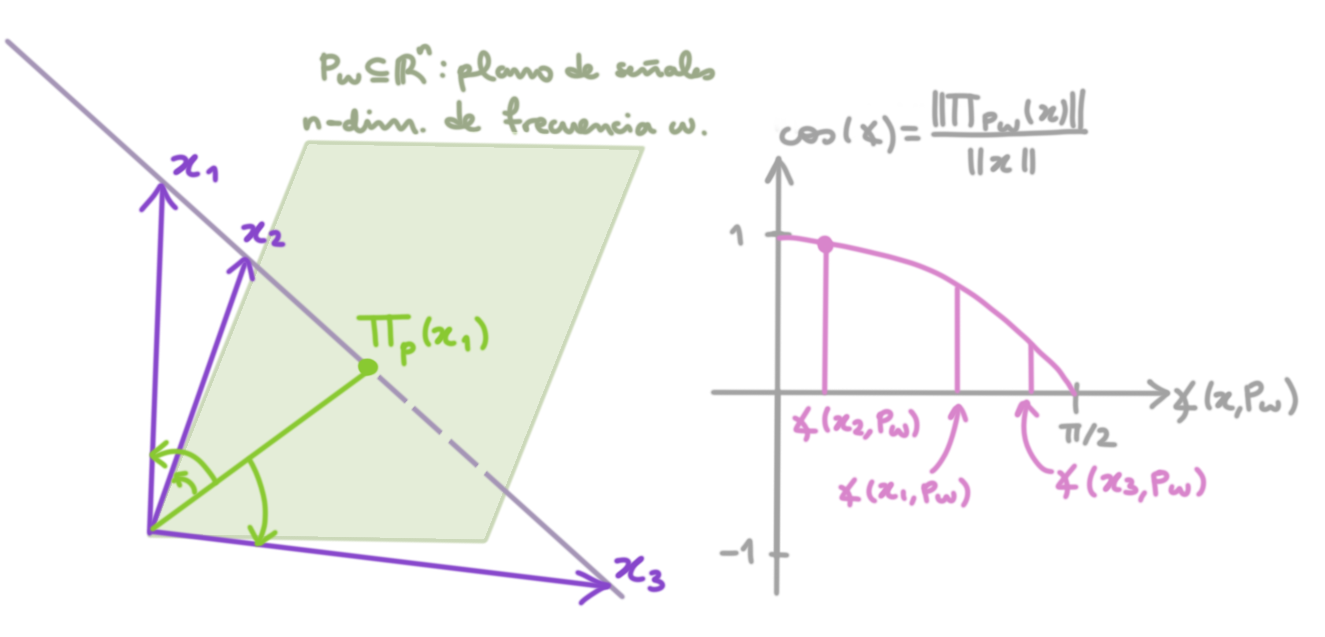
\includegraphics[scale= 1]{20Mar23_1} 
\end{figure}	

Si $x$ es unitaria,
tenemos la relación simplificada 

\begin{equation}
\label{eq1: 20Mar}
cos \left( \measuredangle (x, W) \right) = || \Pi_{W}(x) || 
\hspace{0.5cm} (x \hspace{0.1cm} \text{unitario).}
\end{equation}


\textbf{Usaremos pues, para dar una medida de qué tanto
reacciona una señal $x \in \IR^{n}$ a una frecuencia
$\omega >0$
el número 
$\frac{||\Pi_{P_{n, \omega}}(x)||}{||x||} \in [0,1]$.} \\

\TODO{Deberías notar que sólo hay dos espacios P cuando nomega en n medios Z.}

\begin{defi}
\label{def: final de sigmas}
Sean $n \geq 2$, $\omega \geq 0$. 
Definimos la función $\sigma_{n}(\cdot, \omega)$ para todo 
elemento de $\IR^{n} - \{ 0\}$
como sigue;
\begin{equation}
\label{eq: def sigmas}
	\forall x \in \IR^{n}-\{ 0\}: \hspace{0.2cm}
	\sigma_{n}(x, \omega) = \frac{||\Pi_{P_{n, \omega}}(x)||}{||x||} .
\end{equation}
\end{defi}

Así, fijada una frecuencia $\omega$, 
\begin{itemize}
\item si $\sigma_{n, \omega}(x)$ es ``cercano'' a cero, $\omega$ no
es una frecuencia con la que es razonable aproximar a $x$ (pues $x$ será
cercano a ser ortogonal a toda señal de dimensión $n$ y frecuencia 
$\omega$),  mientras que

\item si $\sigma_{n, \omega}(x)$ es ``cercano'' a uno, también es muy cercano
(hablando en términos de distancia euclídea) a su proyección al espacio
$P_{n, \omega}$, luego $x$ es muy parecido a tener frecuencia $\omega$.
\end{itemize}


Para poder usar las fórmulas
derivadas en la sección 
\ref{ap: Caso particular en el que el subespacio en cuestión es un plano},
debemos de dar una base normalizada del espacio $P_{\omega}$.

\begin{prop}
\label{prop: aaa}
Sean $n \in \IN$, $\omega>0$. Sean los vectores $c_{n, \omega}, 
s_{n ,\omega} \in \IR^{n}$ como se definieron en 
\eqref{eq: coseno omega} y \eqref{eq: seno omega}, 
respectivamente.
\begin{itemize}
	\item Si $\omega \not\in \frac{n}{2} \IZ$, entonces 
	$\{ f_{n, \omega}, g_{n, \omega} \}$, donde

	\begin{equation}
	\label{eq5: 19Marzo}
	f_{n, \omega}=\xi_{n, \omega} c_{n, \omega}
	\in \IR^{n}
	\end{equation}
y 

	\begin{equation}
	\label{eq6: 19Marzo}
	g_{n, \omega}= \eta_{n, \omega} s_{n, \omega}
	\in \IR^{n},
	\end{equation}
con 
\begin{equation}
\label{eq7: 19Marzo}
	\xi_{n, \omega}= 
	\sqrt{2} \cdot \left( n + \frac{sen(2 \pi \omega)
	cos(2 \pi \omega \left(\frac{n-1}{n} \right))}{sen \left(2 \pi 
	\frac{\omega}{n} \right)} \right)^{-\frac{1}{2}} 
\end{equation}
y

	\begin{equation}
	\label{eq8: 19Marzo}
	\eta_{n, \omega}= \sqrt{2} \cdot \left( n - \frac{sen(2 \pi \omega)
	cos(2 \pi \omega \left(\frac{n-1}{n} \right))}{sen \left(2 \pi 
	\frac{\omega}{n} \right)} \right)^{-\frac{1}{2}}.
	\end{equation}

\noindent
es una base normalizada del subespacio $P_{n, \omega} \leq \IR^{n}$
definido en \eqref{eq6: 23Ap}, y,
\item si $\omega \in \frac{n}{2} \IZ$, entonces 
$\{ f_{n, \omega} \}$, con
\begin{equation}
\label{ec: 4: 23ap}
	f_{n, \omega} := \frac{1}{\sqrt{n}}c_{n, \omega}
\end{equation}
es una base normalizada 
del subespacio $P_{n, \omega} \leq \IR^{n}$
definido en \eqref{eq0: 23Ap}.
\end{itemize}
\end{prop}
\noindent
\textbf{Demostración.}
En efecto, por definición del espacio
$P_{n, \omega}$, $\{ c_{n, \omega}, s_{n, \omega} \}$
es una base de este cuando
$\omega \not\in \frac{n}{2}\IZ$, y
$\{ c_{n, \omega}\}$ es base si 
$\omega \in \frac{n}{2}\IZ$,
luego, en ambos casos el conjunto propuesto en efecto
es una base de $P_{n, \omega}$.
En el segundo caso, puesto que
$f_{n, \omega}$ será un vector cuyas entradas serán $1$, o $-1$,
\eqref{ec: 4: 23ap} en efecto es un vector unitario. 
En el primer caso, se han calculado las constantes 
$\xi_{n, \omega}$ y $\eta_{n, \omega}$
dadas en 
\eqref{eq7: 19Marzo} y \eqref{eq8: 19Marzo}
para que $f_{n, \omega}$ y $g_{n, \omega}$
tengan normal uno; puesto que los cálculos son muy
similares a los realizados en la demostración de la proposición
\ref{prop: producto punto entre f y g}, los omitimos.
\QEDB
\vspace{0.2cm}


Conviene también establecer una fórmula para
el producto punto entre 
los vectores $f_{n, \omega}$ y $g_{n, \omega}$
definidos en la proposición \ref{prop: aaa}
cuando $\omega \not\in \frac{n}{2} \IZ$.
Hacemos esto a continuación.

\begin{prop}
\label{prop: producto punto entre f y g}
Fijados $n \geq 2$ y $\omega \geq 0$ con 
$\omega \not\in \frac{n}{2}\IZ$, 
el producto punto entre 
los vectores
$f_{n, \omega}$ y $g_{n, \omega}$, definidos 
\eqref{eq5: 19Marzo} y \eqref{eq6: 19Marzo}
respectivamente, es

\begin{equation}
\label{eq9: 19Marzo}
\langle f_{n, \omega} , g_{n, \omega} \rangle =
\frac{\xi_{n, w} \eta_{n, \omega}}{2} \cdot 
\frac{sen(2 \pi \omega)
sen(2 \pi \omega \left( 1- \frac{1}{n} \right))}{sen \left(2 \pi 
\frac{\omega}{n} \right)}
\end{equation}

\end{prop}
\noindent
\textbf{Demostración.}
Aquí usaremos las siguientes tres igualdades:

\begin{equation}
\label{eq10: 19Marzo}
\forall \alpha \in \IR: \hspace{0.2cm}
sen(2 \alpha) = 2 sen(\alpha) cos(\alpha),
\end{equation}



\begin{equation}
\label{eq11: 19Marzo}
\forall z\in \IR: \hspace{0.2cm}
sen(z)= \frac{e^{iz}-e^{-iz}}{2i},
\end{equation}



\begin{equation}
\label{eq12: 19Marzo}
\forall a \in \IR-\{ 1 \}: \hspace{0.2cm}
\suma{m=0}{n-1}{a^{r}}= \frac{1-a^{n}}{1-a}.
\end{equation}

\noindent
Tenemos que

\begin{align*}
\langle f_{n,\omega} , g_{n, \omega} \rangle = &
\xi_{n, \omega} \eta_{n, \omega} \left\langle 
\left( cos \left( 2 \pi \omega \frac{m }{n} \right) \right)_{0 \leq m \leq N-1} ,  
\left( cos \left( 2 \pi \omega \frac{m }{n}\right) \right)_{0 \leq m \leq N-1} \right\rangle \\
= & \xi_{n, \omega} \eta_{n, \omega} \suma{m=0}{n-1}{
cos \left(2 \pi \omega \frac{m}{n}\right) sen\left( 2 \pi \omega \frac{m}{n}\right)} \\
= & \frac{\xi_{n, \omega} \eta_{n, \omega}}{2}
\suma{m=0}{n-1}{
\left( sen\left( 4 \pi \omega \frac{m}{n}\right) \right)} \\
= & \frac{\xi_{n, \omega} \eta_{n, \omega}}{4i} \suma{m=0}{n-1}{
\left( e^{4 \pi \omega i m/n} - 
e^{-4 \pi \omega i m/n} \right) } \\
= & \frac{\xi_{n, \omega} \eta_{n, \omega}}{4i} 
\left(
\frac{1-e^{4 \pi \omega i }}{1-e^{4 \pi \omega i /N}} - 
\frac{1-e^{-4 \pi \omega i }}{1-e^{-4 \pi \omega i /N}} 
\right) \\
= & \frac{\xi_{n, \omega} \eta_{n, \omega}}{4i} 
\left(
\frac{e^{2 \pi \omega i }}{e^{2 \pi \omega i/n }}
\frac{e^{-2 \pi \omega i }-e^{2 \pi \omega i }}{e^{-2 \pi \omega i/n }-e^{2 \pi \omega i /N}} - 
\frac{e^{-2 \pi \omega i }}{e^{-2 \pi \omega i/n }}
\frac{e^{2 \pi \omega i }-e^{-2 \pi \omega i }}{e^{2 \pi \omega i/n }-e^{2 \pi \omega i /N}} 
\right) \\
= & 
\frac{\xi_{n, \omega} \eta_{n, \omega}}{4i} 
\left(
e^{2 \pi \omega i \left( 1-1/n \right)}
\frac{sen(2 \pi \omega)}{sen(2 \pi \omega /n)} - 
e^{-2 \pi \omega i \left( 1-1/n \right)}
\frac{sen(2 \pi \omega)}{sen(2 \pi \omega /n)}
\right) 
\\
= & 
\frac{\xi_{n, \omega} \eta_{n, \omega}}{4i} 
\frac{sen(2 \pi \omega)}{sen(2 \pi \omega /n)}
\left(
e^{2 \pi \omega i \left( 1-1/n \right)} - e^{-2 \pi \omega i \left( 1-1/n \right)}
\right) \\
= &
\frac{\xi_{n, \omega} \eta_{n, \omega}}{4i} 
\frac{sen(2 \pi \omega)}{sen(2 \pi \omega /n)}
\left(
2i \cdot  sen \left( 2 \pi \omega  \left( 1- \frac{1}{n} \right) \right)
\right)\\
= & 
\frac{\xi_{n, \omega} \eta_{n, \omega}}{2} 
\frac{sen(2 \pi \omega)}{sen(2 \pi \omega /n)}
sen \left( 2 \pi \omega  \left( 1- \frac{1}{n} \right) \right). \\
\end{align*}
\QEDB
\vspace{0.2cm}



\begin{prop}
Sean $n \geq 2$, $\omega \geq 0$. 
Sea $\sigma_{n}(\cdot,\omega): \IR^{n} \longrightarrow [0,1]$
la función definida en \ref{def: final de sigmas}.
Para todo $x \in \IR^{n}-\{ 0 \}$
se tiene que
\begin{itemize}
	\item Si $\omega \not\in \frac{n}{2} \IZ$, entonces
	\begin{equation}
	\label{eq: pi ommm 1}
	 \Pi_{P_{\omega}}(x) = 
\frac{
\langle x, f_{n, \omega} \rangle - \langle f_{n, \omega}, g_{n, \omega} \rangle 
\langle x, g_{n, \omega} \rangle
}
{1-|\langle f_{n, \omega}, g_{n, \omega} \rangle |^{2}  }
f_{n, \omega} +
\frac{
\langle x, g_{n, \omega} \rangle - \langle f_{n, \omega}, g_{n, \omega} \rangle 
\langle x, f_{n, \omega} \rangle
}
{1-|\langle f_{n, \omega}, g_{n, \omega} \rangle |^{2}  }
g_{n, \omega}
	\end{equation}
	y 
	\begin{equation}
	\sigma_{n}(x, \omega) =
	\left(		  
		  \frac{\langle x, f_{n, \omega } \rangle^{2} +  \langle x, g_{n, \omega } \rangle^{2}	
	       -2  \langle x, f_{n, \omega } \rangle \langle x, g_{n, \omega } \rangle \langle f_{n, \omega }, g_{n, \omega } \rangle}{ || x ||^{2} \cdot
	       (1- \langle f_{n, \omega }, g_{n, \omega } \rangle^{2})}	  
\right) ^{1/2},
	\end{equation}
donde $f_{n, \omega}$ y $g_{n, \omega}$ son como en 
\eqref{eq5: 19Marzo} y \eqref{eq6: 19Marzo}, y

\item si $\omega \in \frac{n}{2} \IZ$, entonces 
\begin{equation}
\label{eq: pi ommm 2}
\Pi_{P_{n, \omega}}(x) = \langle x, f_{n, \omega} \rangle f_{n, \omega}
\end{equation}
y 
\begin{equation}
\label{eq: sfklmslsfl}
\sigma_{n}(x, \omega) = \frac{|\langle x, f_{n, \omega} \rangle |}{||x||},
\end{equation}
donde $f_{n, \omega}$ es como en \eqref{ec: 4: 23ap}.
\end{itemize}
\end{prop}


\TODO{a diferencia de la dft, los casos extremos ya no son
estar o no estar, sino ser perpendicular o ser paralelo.}

\subsection{Desfase de la proyección de una señal a espacios monofrecuenciales}

Dada $x \in \IR^{n}$ una señal no cero 
y $\omega > 0$ una frecuencia fija,
buscamos el desfase $\phi \in [0,1]$ que mejor se ajuste a $x$
(c.f. figura \ref{fig: muestreo coseno}).


Puesto que
$\Pi_{P_{n, \omega}}(x)$ (donde $P_{n, \omega}$ es como se definió en 
\eqref{eq6: 23Ap} y \eqref{eq0: 23Ap}, dependiendo si 
$\omega$ es o no elemento de $\frac{n}{2} \IZ$) 
es la señal de frecuencia $\omega$ que está a menor
distancia euclidea de $x$, proponemos usar como
desfase $\phi$ como 
el número entre cero y uno tal que 
\[
\Pi_{P_{n, \omega}}(x) = A (cos(2 \pi \omega t -  2 \pi \phi ))_{t \in I_{n}}
\]
para alguna amplitud $A$. \\

Fijada entonces una frecuencia $\omega$, nos interesa encontrar
el desfase (normalizado) $\phi$ y la amplitud $A$ del sinusoide
de frecuencia $\omega$ cuya discretización en $I_{n}$ es la proyección
ortogonal $\Pi_{P_{n, \omega}}(x)$. \\


Primero abordemos el caso en el que
$\omega \not\in \frac{n}{2} \IZ$. 

Como los vectores $f_{n, \omega}$ y $g_{n, \omega}$ 
definidos en \eqref{eq5: 19Marzo} y \eqref{eq6: 19Marzo}
son unitarios y linealmente independientes (c.f. proposición
\ref{prop: aaa}),
podemos usar la ecuación \eqref{eq0: 24ap}
para escribir a la proyección de $x$ en $P_{\omega}$ como sigue


\begin{equation}
\label{eq3: 20Marzo}
\Pi_{P_{\omega}}(x)= c (cos (2 \pi \omega t))_{t \in I_{n}} + d 
(sin (2 \pi \omega t))_{t \in I_{n}},
\end{equation}
donde

\begin{equation}
\label{eq4: 20Marzo}
c= \frac{
\langle x, f_{n, \omega} \rangle - \langle f_{n, \omega}, g_{n, \omega} \rangle
\langle x, g_{n, \omega} \rangle
}{1-\langle f_{n, \omega}, g_{n, \omega} \rangle^{2}} \xi_{n, \omega}
\end{equation}
y
\begin{equation}
\label{eq5: 20Marzo}
d= \frac{
\langle x, g_{n, \omega} \rangle - \langle f_{n, \omega}, g_{n, \omega} \rangle
\langle x, f_{n, \omega} \rangle
}{1-\langle f_{n, \omega}, g_{n, \omega} \rangle^{2}} \eta_{n, \omega}.
\end{equation}

\noindent 
Nos conviene más reescribir a \eqref{eq3: 20Marzo} como
\begin{equation}
\label{eq6: 20Marzo}
\Pi_{P_{n, \omega}}(x)= 
\sqrt{c^{2}+d^{2}}
\left[
C (cos (2 \pi \omega t))_{t \in I_{n}} +
D (sen (2 \pi \omega t))_{t \in I_{n}} 
\right],
\end{equation}

\noindent 
donde

\begin{equation}
\label{eq3: 28Marz23}
C:= \frac{c}{\sqrt{c^{2}+d^{2}}} \hspace{0.2cm} \text{y}
\hspace{0.2cm} D:= \frac{d}{\sqrt{c^{2}+d^{2}}},
\end{equation}
\noindent 
pues, como $C^{2} + D^{2}=1$, existe un único
$\phi \in [0,1[$ tal que
\begin{equation}
\label{eq7: 20Marzo}
C= cos(2 \pi \phi), \hspace{0.2cm} 
D= sin(2 \pi \phi).
\end{equation}

\noindent 
Sustituyendo \eqref{eq7: 20Marzo} en \eqref{eq6: 20Marzo},
llegamos a que

\begin{align*}
\Pi_{P_{n, \omega}}(x) = & 
\sqrt{c^{2}+d^{2}} \left[
cos(2 \pi \phi) \cdot (cos (2 \pi \omega t))_{t \in I_{n}} +
sin(2 \pi \phi) \cdot (sin (2 \pi \omega t))_{t \in I_{n}} 
\right] \\
= & 
\sqrt{c^{2}+d^{2}} 
(cos(2 \pi \phi) \cdot cos (2 \pi \omega t) +
sin(2 \pi \phi) \cdot sin (2 \pi \omega t) )_{t \in I_{n}} \\
= & 
\sqrt{c^{2}+d^{2}} 
(cos(2 \pi \omega t - 2 \pi \phi))_{t \in I_{n}}.
\end{align*}

\noindent
Además, de \eqref{eq7: 20Marzo} y \eqref{eq3: 28Marz23}
se deduce que
\begin{equation}
\label{eq: desfase phi 1}
\phi =
\begin{cases}
\frac{tan^{-1}(d/c) }{2 \pi}  \hspace{0.4cm}    \text{   si }   d, c > 0,  \\
\frac{tan^{-1}(d/c) + \pi }{2 \pi} \hspace{0.2cm}  \text{si }  d, c < 0,  \\
\frac{tan^{-1}(d/c) + \pi }{2 \pi} \hspace{0.2cm}  \text{si }  d>0,  c < 0,  \\
\frac{tan^{-1}(d/c) + 2\pi }{2 \pi} \hspace{0.2cm}  \text{si }  d>0,  c < 0. 
\end{cases}
\end{equation}

Hemos probado el siguiente
\begin{teo}
Sean $n \geq 2$ y $\omega > 0$ con $\omega \not\in \frac{n}{2}\IZ$.
Si $P_{n, \omega}$ es el subespacio de $\IR^{n}$ definido como 
en \eqref{eq6: 23Ap}, entonces, para todo 
$x \in \IR^{n}$ no cero, se tiene que
\begin{equation}
\label{ec: desfase explicito 1}
\Pi_{P_{n, \omega}} (x) = \sqrt{c^{2}+d^{2}} \cdot (
cos (2 \pi \omega t - 2 \pi \phi)
)_{t \in I_{n}} \in \IR^{n},
\end{equation}

\noindent
donde 
$c$ y $d$ son como en \eqref{eq4: 20Marzo} y 
\eqref{eq5: 20Marzo}, respectivamente, y $\phi$ está 
dado por \eqref{eq: desfase phi 1}.
\end{teo}
Observe que tenemos una fórmula para obtener a
la frecuencia y amplitud de $\Pi_{P_{n, \omega}}(x)$
usando sólamente los datos
\[
\langle x, f_{n, \omega} \rangle, \hspace{0.2cm}
\langle x, g_{n, \omega} \rangle \hspace{0.1cm} \text{y} \hspace{0.1cm}
\langle f_{n, \omega}, g_{n, \omega} \rangle.
\]

El resultado análogo para cuando $\omega \in \frac{n}{2}\IZ$
es más fácil de establecer, pues en este caso
el espacio monofrecuencia $P_{n, \omega}$ es una recta.

\begin{teo}
Sean $n \geq 2$ y $\omega > 0$ con $\omega \in \frac{n}{2}\IZ$.
Si $P_{n, \omega}$ es el subespacio de $\IR^{n}$ definido como 
en \eqref{eq0: 23Ap}, entonces, para todo 
$x \in \IR^{n}$ no cero, se tiene que
\begin{equation}
\label{ec: desfase explicito 2}
\Pi_{P_{n, \omega}} (x) = 
\frac{1}{\sqrt{n}} \langle x, f_{n, \omega} \rangle
\cdot (cos (2 \pi \omega t))_{t \in I_{n}} \in \IR^{n}.
\end{equation}
\end{teo}
\noindent
\textbf{Demostración.}
En efecto, según \eqref{eq: pi ommm 2} y 
\eqref{ec: 4: 23ap},
se tiene que
\begin{align*}
\Pi_{P_{n, \omega}} (x) = & 
\langle x, f_{n, \omega} \rangle f_{n, \omega} \\
= & \langle x, f_{n, \omega} \rangle \frac{1}{\sqrt{n}} c_{n, \omega} \\
= & \frac{1}{\sqrt{n}} \langle x, f_{n, \omega} \rangle
\cdot (cos (2 \pi \omega t))_{t \in I_{n}} \in \IR^{n}.
\end{align*}

\QEDB
\vspace{0.2cm}

\chapter{Análisis espectrales: resultados numéricos}
\label{chap: resultados numericos analisis espectrales}

Después de todo lo expuesto en las secciones anteriores, tenemos
ya dos alternativas para graficar el espectro
de una señal $x \in \IR^{n}$.

\begin{itemize}
	\item Usando la transformada discreta de Fourier
	(c.f. sección \ref{sec: TDF}), el espectro de
	una señal $x$ es la gráfica de las frecuencias
	enteras dadas (dependiendo de la 
	paridad de $n$) por las
	tablas 6.1 y 6.2
	versus los coeficientes
	$\tau_{n}(x)$ definidos en
	\ref{def: taus}.
	\TODO{Puesto que hacer un análisis con la
	DFT significa expresar a $x$ como una suma
	ponderada de muestreos de senos y cosenos
	de algunas frecuenicas enteras,...}
	
	\item Si, para hacer un análisis espectral, se usan
	las ideas propuestas en 
	la sección
	\ref{sec: metodologia para realizar un analisis espectral que considere frecuencias arbitrarias}, entonces, dado un rango de frecuencias 
	$\omega$,
	el espectro de $x$ es la gráfica de 
	las frecuencias $\omega$ versus	
	los coeficientes
	$\sigma_{n}(x, \omega)$.
	

\TODO{a diferencia de la dft, los casos extremos ya no son
estar o no estar, sino ser perpendicular o ser paralelo a su
representante del espacio monofrecuencial.}
\end{itemize}

Espectro cero: el de TDF
Espectro uno: el de espacios monofrecuenciales

\begin{figure}[H]
	\sidecaption{
	Ejemplo de los espectros resultantes
	de los dos métodos de análisis.
	\label{fig: espectro 1 }
	}
	\centering
	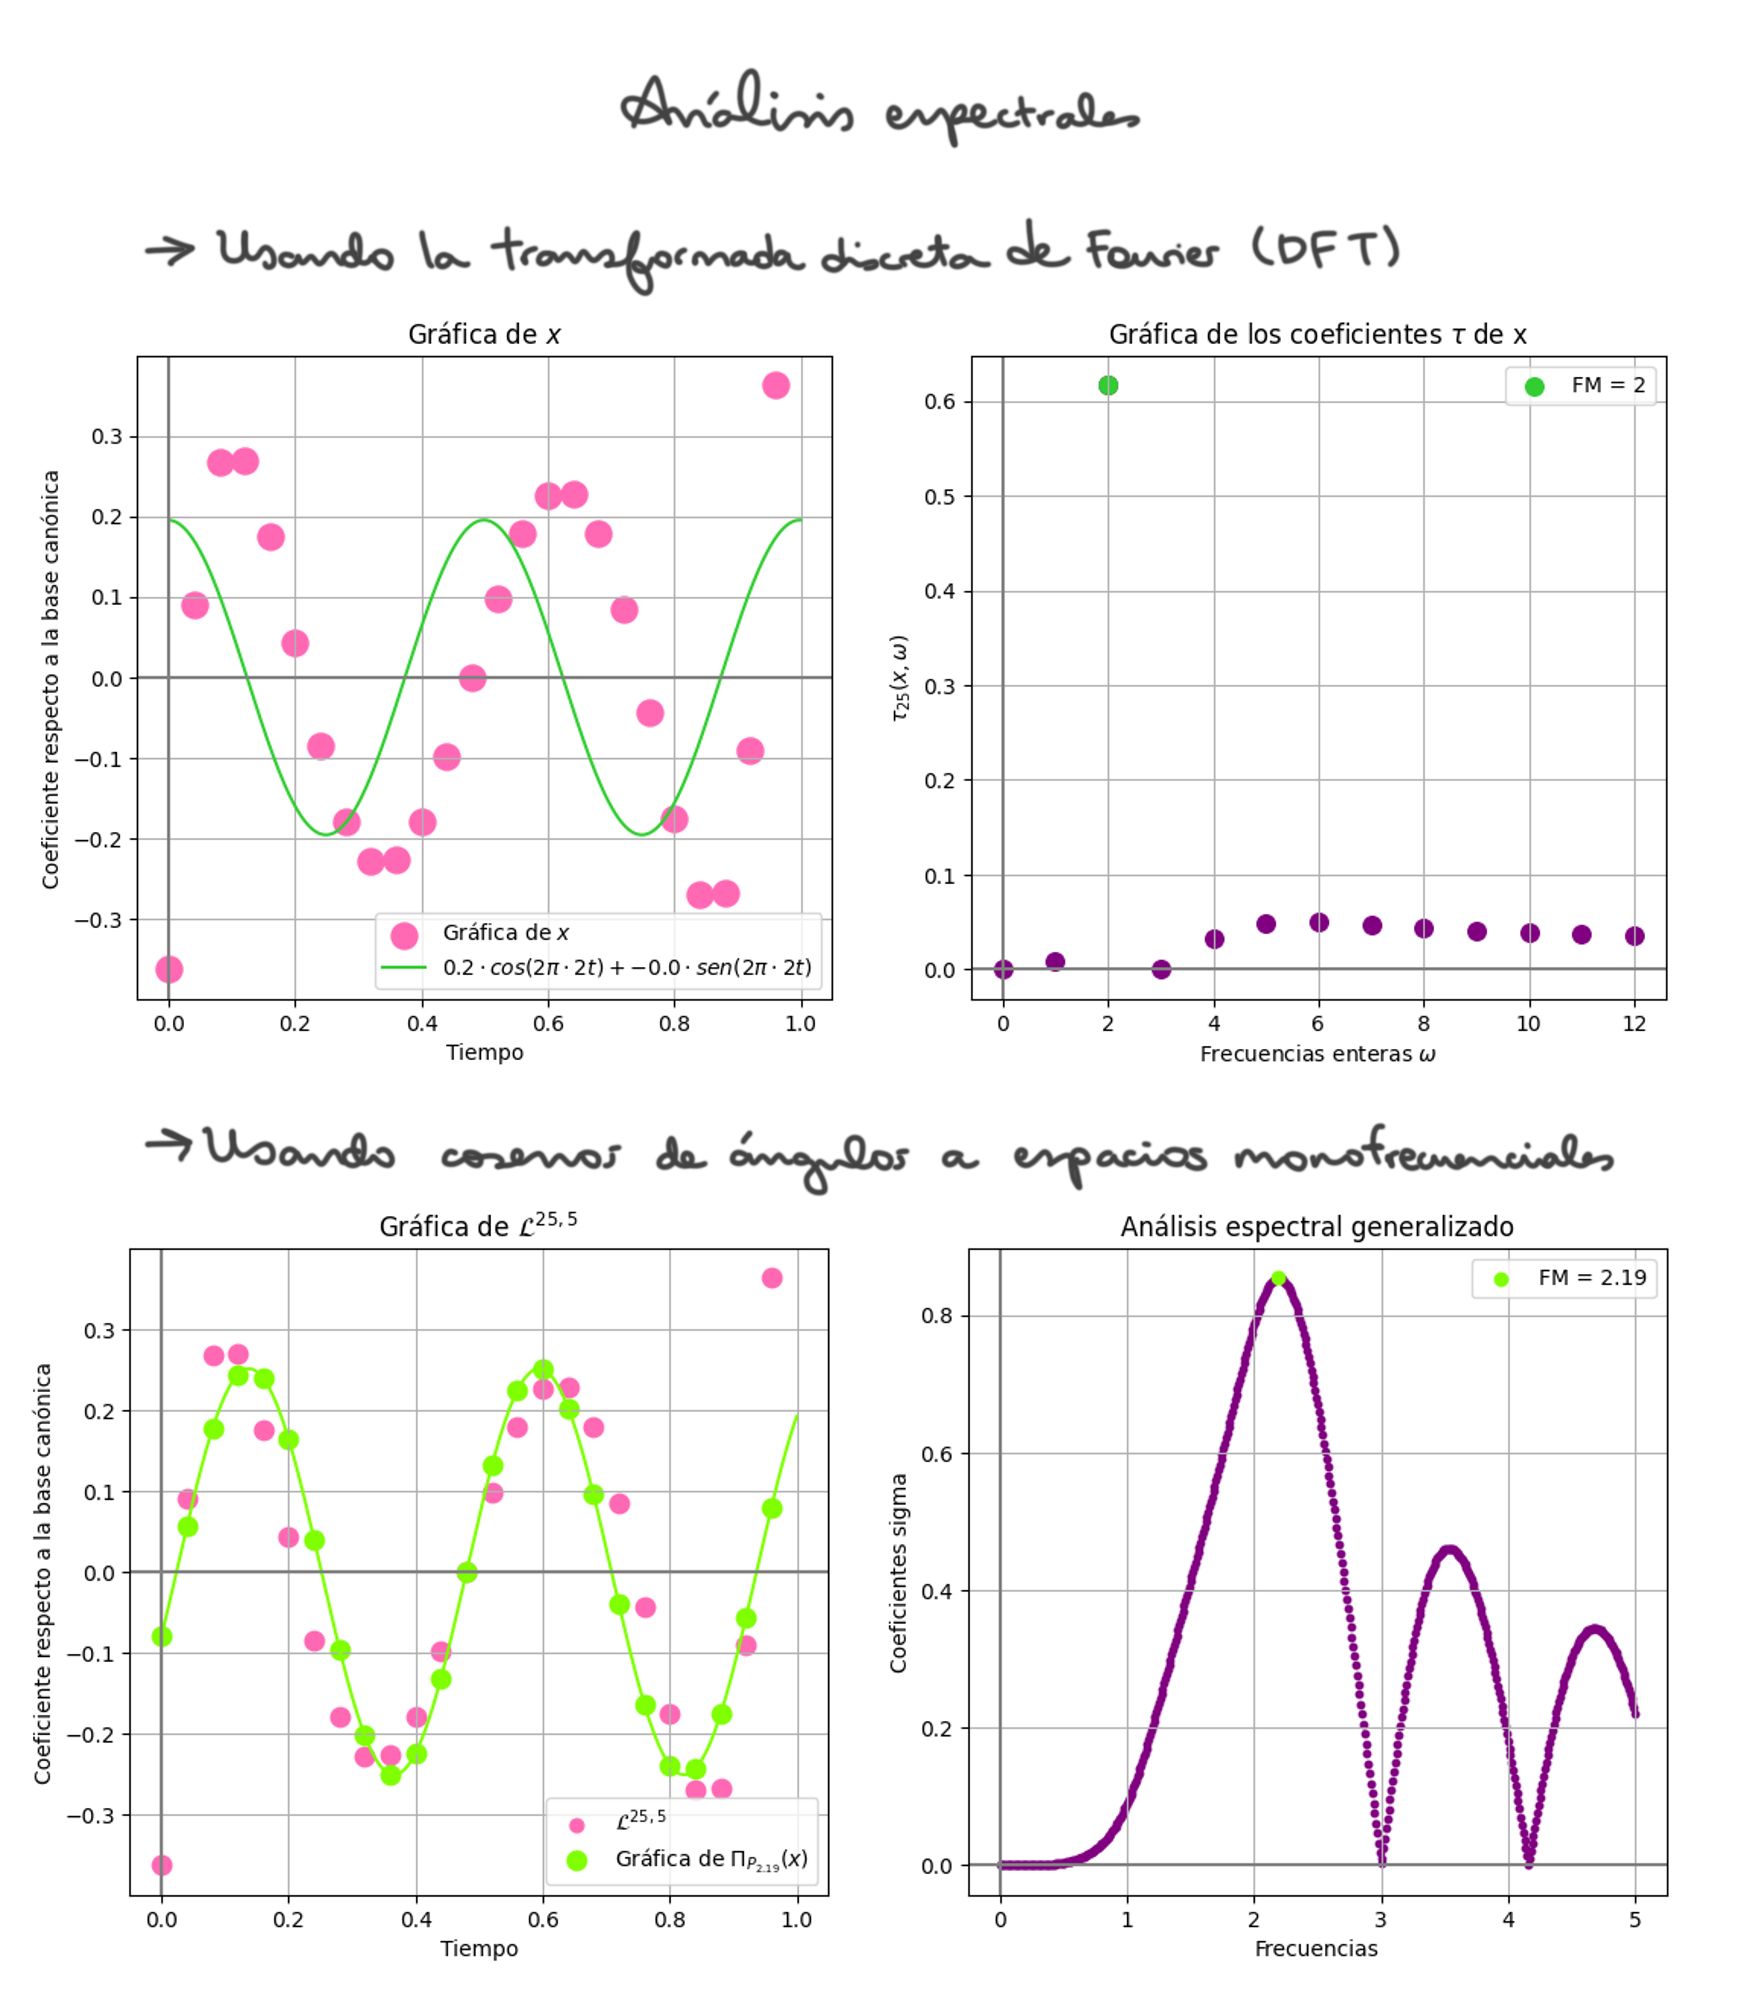
\includegraphics[scale = 1]{ejemplo_analisisEspectrales} 
\end{figure}	

\section{Lista de preguntas a responder usando los resultados numéricos}

\begin{notacion}
Dados los espectros cero y uno de $\cali{L}^{n,k}$, si
$FM_{i}$ 
(para $i=0,1$)
es la frecuencia $\omega$ en la que el espectro 
$i$ alcanza su punto máximo.
\TODO{cambia esto en los cpódgios}
\end{notacion}


Enlistamos las preguntas que nos interesa considerar
(formuladas de manera general, pero que comprobaremos o refutaremos
numéricamente para dimensiones hasta $n=70$, pues para dimensiones
más grandes los errores computacionales son demasiado grandes
como para obtener conclusiones fiables, \TODO{revisa lo que tiene que
decir al respecto el libro de data science!}).

Vamos a responder estas preguntas con gráficas!

La primera pregunta es una reformulación de la 
hipótesis \ref{ref: hipotesis}. Hacemos dos preguntas
más para afinar.

\begin{itemize}
\item \textbf{Pregunta 1}: 
Para cualesquiera $n \geq 2$ y $0 \leq k \leq n-1$,
¿ocurre que las frecuencias máximas
$FM_{0}$ y $FM_{1}$ son cercanas a $\frac{k}{2}$?

\begin{figure}[H]
	\sidecaption{
	\TODO{Voy a responder esta con algunas imágenes de espectros como esta.}
	\label{fig: ejemplo_pregunta1}
	}
	\centering
	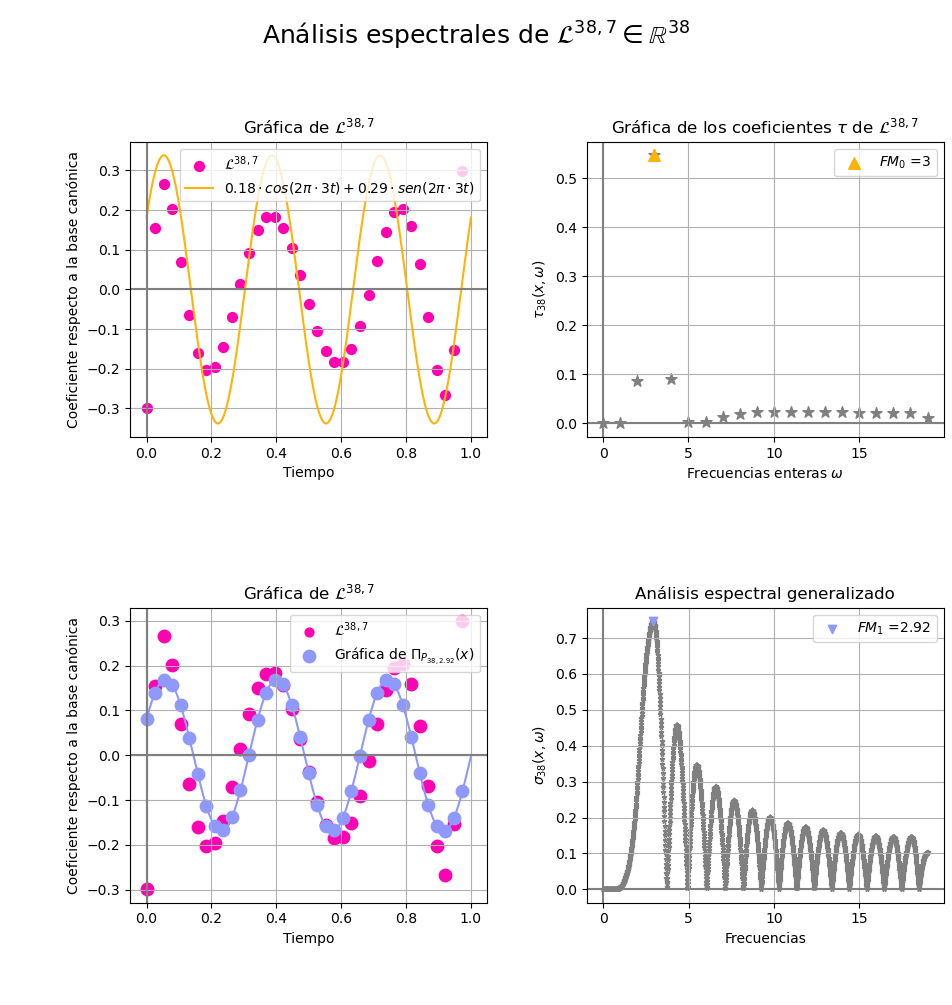
\includegraphics[scale = 0.5]{./estudios_espectrales/ejemplo_pregunta1} 
\end{figure}	

\item \textbf{Pregunta 2}: ¿En efecto dependen $FM_{0}$ y $FM_{1}$ sólo
de $k$ y no de $n$?

\begin{figure}[H]
	\sidecaption{
	\TODO{Voy a responder esta con algunas imágenes de espectros como esta.}
	\label{fig: ejemplo_pregunta2}
	}
	\centering
	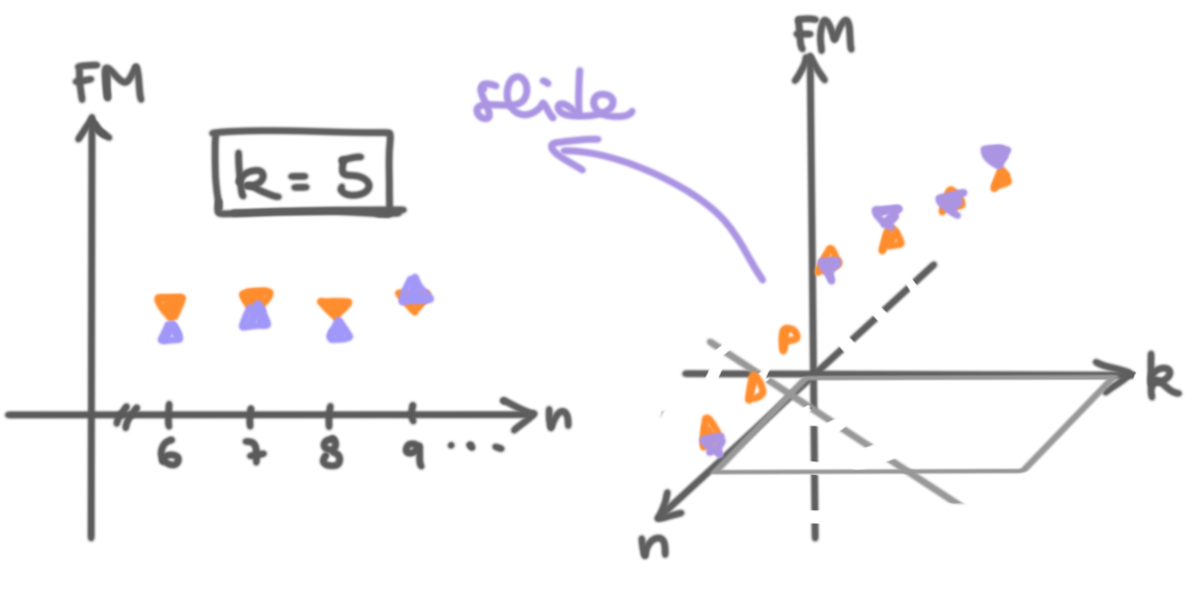
\includegraphics[scale = 1]{./estudios_espectrales/ejemplo_pregunta2} 
\end{figure}	

\item \textbf{Pregunta 3}: ¿Los parámetros $(m,b)$ de pendiente y ordenada al 
origen de las rectas de mínimos cuadrados (RMC) de las gráficas 
de FM para un $n$ fijo son parecidos? ¿En dónde se concentran?
\TODO{reformula mejor. Esta pregunta es para mejor la estimación dada
en la hipótesis!}
\begin{figure}[H]
	\sidecaption{
	\TODO{Voy a responder esta con algunas imágenes de espectros como esta.}
	\label{fig: ejemplo_pregunta3}
	}
	\centering
	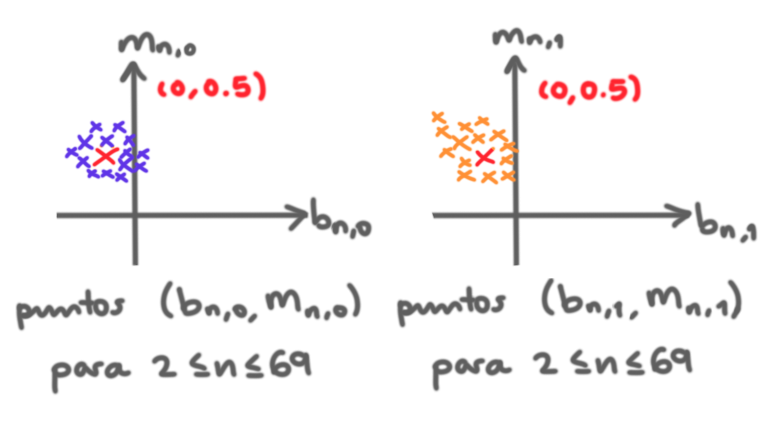
\includegraphics[scale = 1]{./estudios_espectrales/ejemplo_pregunta3} 
\end{figure}	
\end{itemize}

Note que las preguntas 2 y 3 son más bien globales
(y las respondo numéricamente con los datos calculados en 
la función \texttt{analisis$\_$espectralPDL$\_$global}).